\documentclass[preprint,12pt]{elsarticle}

\usepackage[T1]{fontenc}
\usepackage{amsmath,amssymb,amsthm}
\usepackage{booktabs}
\usepackage{array}
\usepackage{tikz}
\usetikzlibrary{arrows.meta,positioning}
\usepackage{xcolor}
\usepackage{listings}
\usepackage[expansion=false]{microtype}
\setlength{\emergencystretch}{1.5em}
\usepackage{hyperref}
\hypersetup{colorlinks=true,linkcolor=blue!50!black,citecolor=blue!50!black,urlcolor=blue!50!black}

% ---------- theorem environments ----------
\theoremstyle{plain}
\newtheorem{theorem}{Theorem}[section]
\newtheorem{proposition}[theorem]{Proposition}
\newtheorem{corollary}[theorem]{Corollary}
\newtheorem{lemma}[theorem]{Lemma}
\theoremstyle{definition}
\newtheorem{definition}[theorem]{Definition}
\newtheorem{example}[theorem]{Example}
\newtheorem{remark}[theorem]{Remark}

% ---------- macros ----------
\newcommand{\en}{\mathit{en}}
\newcommand{\st}{\mathit{start}}
\newcommand{\ovr}{\mathit{over}}
\newcommand{\stp}{\mathit{end}}
\newcommand{\eff}{\mathit{eff}}
\newcommand{\acq}{\mathit{acq}}
\newcommand{\rel}{\mathit{rel}}
\newcommand{\id}{\mathit{id}}
\newcommand{\conf}{\mathrel{\#}}
\newcommand{\B}[1]{\mathsf{B}#1}
\newcommand{\E}[1]{\mathsf{E}#1}
\newcommand{\steparrow}[1]{\mathrel{[#1\rangle}}
\newcommand{\istep}[1]{\xrightarrow{#1}}
\newcommand{\BE}[1]{#1^{\mathit{BE}}}
\newcommand{\D}{\mathcal{D}}
\newcommand{\G}{\mathcal{G}}
\newcommand{\Coh}{\mathit{coherent}}
\newcommand{\enB}[2]{\mathit{enB}_{#1}(#2)}
\newcommand{\enE}[2]{\mathit{enE}_{#1}(#2)}
\newcommand{\wprec}{\sqsubset}
\newcommand{\IO}{\mathit{IO}}
\newcommand{\ext}{\mathit{ext}}
\newcommand{\lean}[1]{\texttt{#1}}

\lstdefinelanguage{lean}{
  keywords={theorem,lemma,def,structure,inductive,where,fun,by,decide,intro,simp,exact,example,instance,deriving,abbrev},
  sensitive=true, comment=[l]{--}, morestring=[b]"}
\lstset{language=lean,basicstyle=\ttfamily\footnotesize,keywordstyle=\bfseries,columns=fullflexible,
  frame=single,framerule=0.3pt,xleftmargin=4pt,xrightmargin=4pt,
  literate={→}{{$\to$}}1 {∀}{{$\forall$}}1 {∃}{{$\exists$}}1 {↔}{{$\leftrightarrow$}}1 {¬}{{$\neg$}}1 {∧}{{$\wedge$}}1 {∨}{{$\vee$}}1 {∈}{{$\in$}}1 {∉}{{$\notin$}}1 {≠}{{$\neq$}}1 {⊆}{{$\subseteq$}}1 {×}{{$\times$}}1 {∘}{{$\circ$}}1 {∅}{{$\emptyset$}}1 {≤}{{$\le$}}1}

\journal{Theoretical Computer Science}

\begin{document}

\begin{frontmatter}

\title{Actions Take Time:\\ Transparency Conditions for the Interval Semantics of Guarded Actions}

\author{Mohammed A. Alqarni}
\ead{alqarni@uj.edu.sa}
\address{Department of Software Engineering, University of Jeddah, Jeddah, Saudi Arabia}

\begin{abstract}
An action that takes time has a beginning and an end, and other actions may begin and end in between; an interval semantics describes a system by such sequences, observed as interval orders. We ask what a condition of an action may safely observe while other actions are in flight, in guarded action systems with durative actions: conditions checked at the beginning, held throughout, or checked at the end, and a \emph{visibility discipline} fixing which part of an effect becomes visible at each end. For conditions checked at the beginning, interval semantics agrees with step semantics exactly when no beginning changes whether an independent action is enabled, and the run set is determined by its interval orders exactly under a strictly weaker swap condition; both are decided by two-action witnesses, and the least repair is computed. This explains an asymmetry between inhibitor and activator nets. For conditions held throughout or checked at the end, agreement of interval step sequences with interval sequences is characterised by transparency of beginnings and of endings, and the nine placements of conditions and effects are classified: exactly two are sound for every system, they are mirror images, and among the disciplines publishing at one end exactly these can require concurrency. Over-all conditions need conflicts, with no least repair in general. Without temporal gaps, interval reachability is sequential. Conditions held over an interval generate constraints between endings and between beginnings that precedence and weak precedence cannot express. All theorems and examples are checked in Lean~4.
\end{abstract}

\begin{keyword}
concurrency \sep interval orders \sep step semantics \sep durative actions \sep inhibitor nets \sep temporal planning \sep Lean~4
\end{keyword}

\end{frontmatter}

% =====================================================================
\section{Introduction}
\label{sec:intro}

In most semantics of concurrent systems an action is an event: it happens at a point, and the state before it determines whether it may happen. Many actions are not like this. A transaction, a tool call issued by a software agent, a step of a plan with a duration, a transition of a Petri net that is fired non-atomically: each has a beginning and an end, and between the two, other actions begin and end. Wiener observed in 1914 that the observations of a single observer of such behaviour form an \emph{interval order}~\cite{Wiener1914}; Fishburn showed that every interval order on a finite set is represented by a sequence in which each element appears once as a beginning and once as an end~\cite{Fishburn1970}; and Janicki and Koutny made interval orders a basis for the semantics of concurrency~\cite{JanickiKoutny1993}. An \emph{interval semantics} describes a system by the sequences of beginnings and endings it can produce.

Once actions have duration, a condition attached to an action acquires a time at which it is evaluated. The planning language PDDL2.1 distinguishes three placements~\cite{FoxLong2003}: a condition may be required \emph{at the start} of the action, \emph{at the end}, or \emph{over all} of its duration. A second parameter is when the effects of an action become visible to others: at the start, at the end, or part at each. Together the two parameters decide what a condition observes. If an action removes a resource when it begins and another action tests for the absence of that resource, the second action sees the removal before the first has finished; if the removal becomes visible only at the end, it does not. Our earlier work on Petri nets with inhibitor arcs met this question in a concrete form~\cite{AlqarniJanicki2015,AlqarniJanicki2018,Alqarni2016}: the natural interval translation of an inhibitor net admits behaviours the net forbids, and the remedy was a second inhibitor arc from every transition that consumes the inhibiting token. Janicki later found that the analogous translation of activator nets, where a transition tests for the presence of a token, is neither sound nor consistent with step semantics, while the inhibitor translation is both~\cite{Janicki2019}. Chatain, Haar, Koutny and Schwoon gave a different translation for read arcs, in which a consumed token remains readable until its consumer ends~\cite{ChatainHaarKoutnySchwoon2015}. Each of these works fixes one net class and one construction. This paper abstracts from both and asks the general question: for which placements of conditions and effects does an interval semantics agree with the semantics in which actions are events, and when it does not, what exactly goes wrong?

\paragraph{The model}
We work with \emph{guarded action systems} with durative actions. The state space is arbitrary. An action $a$ has three conditions, $\st_a$, $\ovr_a$ and $\stp_a$, and an effect split into a part $\acq_a$ applied when $a$ begins and a part $\rel_a$ applied when it ends; a symmetric conflict relation says which actions may not overlap, and the parts of independent actions commute. The split of the effect is the \emph{visibility discipline}. The \emph{committed} discipline publishes everything at the end; the \emph{start-only} discipline publishes everything at the beginning; a \emph{consuming} discipline removes what an action consumes when it begins and adds what it produces when it ends. Runs are sequences of beginnings and endings from a \emph{configuration}, a state together with the set of actions in flight, and a run is valid when every condition holds where it is required. Elementary nets with inhibitor arcs, activator (read) arcs under either of the two constructions mentioned above, and PDDL2.1 durative actions without numeric fluents are instances.

\paragraph{Part A: conditions at the start}
When all conditions are checked when the action begins, a step of pairwise independent actions is represented by the words in which all its beginnings precede all its endings. The step semantics and the interval semantics agree, in the sense that a step fires from a state exactly when every such word runs there and some word runs only if the step fires, if and only if the discipline is \emph{acquire-transparent}: the beginning of an action never changes whether an independent action is enabled (Theorem~\ref{thm:A-char}). The run set is determined by the interval orders of its runs, Janicki's soundness, if and only if a strictly weaker \emph{swap condition} holds (Theorem~\ref{thm:A-sound}). Both failures have two-action witnesses, and the least conflict relation restoring either property is the set of pairs with a witness (Corollaries~\ref{cor:A-repair} and~\ref{cor:A-swaprepair}). Under the committed discipline every system is transparent; under a consuming discipline a condition that tests for absence breaks transparency as soon as an independent action consumes the resource tested. This is the asymmetry of~\cite{Janicki2019}: the inhibitor construction of~\cite{AlqarniJanicki2015} is the committed discipline for the purposes of guards, which we make precise (Proposition~\ref{prop:double}), while the activator construction is a consuming one. The split construction of~\cite{ChatainHaarKoutnySchwoon2015} is the committed discipline for positive conditions read at the start, and under it activator nets regain both properties.

\paragraph{Part B: conditions throughout and at the end}
When a condition must hold throughout an action, blocks of actions are no longer the right unit of comparison, because an ending of one action can falsify the over-all condition of another while both are in flight. We compare the interval semantics with steps of \emph{events}: sets of beginnings of independent actions, or sets of endings. Such homogeneous event steps are the step side of Janicki's interval step sequences~\cite{Janicki2019}, and the natural question is when every enabled step can be fired in every order. The answer is \emph{event transparency}: no beginning changes whether an independent action can begin, and no ending changes whether another action can end (Theorem~\ref{thm:B-char}); again with a forward and a backward half, two-action witnesses, and a swap condition for soundness (Theorem~\ref{thm:B-sound}). Part A is the special case of trivial over-all and end conditions (Proposition~\ref{prop:bridge}). The two conditions let us classify the nine combinations of where conditions are read and where effects are published (Table~\ref{tab:cells}). Exactly two combinations are sound and consistent for every system, conditions at the start with effects at the end, and conditions at the end with effects at the start; they are mirror images, and in both every interaction between a condition of one action and an effect of another relates a beginning to an ending. Every other combination has a two-action counterexample. In particular, conditions that must hold over all of an action are unsound under every discipline; the interference is between two endings under the committed discipline and between two beginnings under the others. What repairs them is a conflict; we give a repair (Theorem~\ref{thm:lock}) and show by a three-action example that, unlike in Part~A, no least repair exists in general (Remark~\ref{rem:noleast}).

\paragraph{Required concurrency and structures}
Among the six combinations that publish effects at one end, the two sound ones are exactly the two in which an action can have a \emph{temporal gap} in the sense of Cushing, Kambhampati, Mausam and Weld~\cite{CushingEtAl2007}. We prove, for arbitrary state spaces, that if no action has a temporal gap then every state reachable by overlapping actions is reachable by non-overlapping ones (Theorem~\ref{thm:nogap}), the per-system form of their Theorem~6, and we give two-action witnesses for each kind of gap. So interval orders are a safe abstraction of the run set precisely in the cases where interval semantics is also indispensable. Finally we look at the histories that the two unsound kinds of interference produce. A constraint between two beginnings, or between two endings, cannot be expressed by the relations of precedence and weak precedence on which the interval order structures of Janicki and Koutny~\cite{JanickiKoutny1993} and the combined structures of Janicki, Kleijn, Koutny and Mikulski~\cite{JanickiKleijnKoutnyMikulski2024} are built. With two actions this shows as a run set that its interval orders do not determine; with three actions, as a history that is not the set of extensions of any such structure (Propositions~\ref{prop:beginbegin} and~\ref{prop:endend}). Two further examples calibrate the notion of history: the review and release net of our earlier work shows that all runs between two states may merge two causal histories whose union is not representable although each is, and a disjunctive condition shows that representability depends on the language of conditions and not only on the discipline.

\paragraph{Mechanisation}
Every theorem and every example in the paper, and every proposition except the one about nets (Proposition~\ref{prop:double}), is proved in Lean~4~\cite{deMouraUllrich2021} on top of Mathlib~\cite{Mathlib2020}; Corollary~\ref{cor:blocks} is proved on paper. The general results are ordinary proofs; the finite examples are checked by complete enumeration inside the kernel, never by testing selected traces. Section~\ref{sec:lean} maps each statement to its formal counterpart and lists the axioms used. The development, the toolchain versions and a build command are in the companion repository.

\paragraph{Contributions}
\begin{enumerate}
\item A model of durative guarded actions over arbitrary state, with three condition placements and a visibility discipline, that has elementary inhibitor nets, activator nets under both existing constructions, and propositional PDDL2.1 durative actions as instances (Section~\ref{sec:model}).
\item For conditions at the start: the characterisation of agreement with step semantics by acquire-transparency, of soundness by the swap condition, the two-action witnesses, the least repair, and the explanation of the inhibitor versus activator asymmetry (Section~\ref{sec:partA}).
\item For conditions throughout and at the end: event transparency, the characterisation of agreement between interval step sequences and interval sequences, the soundness characterisation, the lock theorem with its repair and the absence of a least repair, and the classification table with its two general theorems and seven counterexamples (Section~\ref{sec:partB}).
\item The temporal-gap theorem for arbitrary state spaces and the witnesses for required concurrency (Section~\ref{sec:gap}).
\item The two obstructions, between beginnings and between endings, to representing histories by precedence and weak precedence, together with the two calibrating examples (Section~\ref{sec:structures}).
\item A Lean~4 development covering all of the above (Section~\ref{sec:lean}).
\end{enumerate}

\paragraph{What is not claimed}
The conditions we characterise are structural: they say when the splitting of actions into beginnings and endings is faithful to the step semantics, and when the interval orders of the runs are a safe abstraction of the runs. They do not say that a condition checked at the start remains true until the action takes effect; that is a different policy. Written as an over-all condition it is enforced by the blocking reading of the semantics, but Section~\ref{sec:partB} shows that no choice of discipline then keeps steps and interval orders faithful without conflicts. We return to this distinction when we read the results for tool-using agents in Section~\ref{sec:agents}, where the queue example of Part~A and the revocation example of Part~B stand side by side.

\paragraph{Relation to the author's earlier work}
The interval semantics of inhibitor nets in~\cite{AlqarniJanicki2015,Alqarni2016,AlqarniJanicki2018} is one instance of the present model, and two of its results reappear here as special cases: the step-conservativity of the double-arc construction, which is Proposition~3 of~\cite{AlqarniJanicki2018} and is due to Janicki and Yin~\cite{JanickiYin2017}, and the existence of behaviour reachable only through overlapping actions, exhibited there by the net $N_{io}$. Everything beyond these two facts, in particular the characterisations, the classification, the gap theorem and the structural obstructions, is new, as is the mechanisation.

% =====================================================================
\section{Preliminaries}
\label{sec:prelim}

\paragraph{Interval orders}
A strict partial order $\prec$ on a set $X$ is an \emph{interval order} if $a \prec b$ and $c \prec d$ imply $a \prec d$ or $c \prec b$, for all $a, b, c, d \in X$. Interval orders are exactly the orders of intervals of the real line under ``ends before the other begins''.

\begin{theorem}[Fishburn~\cite{Fishburn1970}]
\label{thm:fishburn}
A strict partial order $\prec$ on a finite set $X$ is an interval order if and only if there is a total order $\lhd$ on $\{\B{x}, \E{x} \mid x \in X\}$ with $\B{x} \lhd \E{x}$ for every $x$ and $x \prec y \iff \E{x} \lhd \B{y}$ for all $x, y$.
\end{theorem}

We call a word over the symbols $\B{x}, \E{x}$, in which each symbol of $X$ occurs once and every $\B{x}$ precedes its $\E{x}$, a \emph{complete word} over $X$, and write $\prec_w$ for the interval order it represents. Two complete words represent the same interval order exactly when they agree on the relative position of every $\E{x}$ and $\B{y}$ with $x \neq y$; they may differ in the order of adjacent beginnings and of adjacent endings.

A strict partial order is \emph{stratified} if incomparability together with equality is an equivalence relation. Stratified orders are the orders generated by step sequences, sequences of sets of simultaneous events, and every stratified order is an interval order; the order with $a \prec b$ and $c$ incomparable to both is an interval order that is not stratified.

\paragraph{Precedence and weak precedence}
Janicki and Koutny describe a concurrent history, a set of equivalent observations, by two relations on the events~\cite{JanickiKoutny1993,JanickiKoutny1997}: \emph{precedence} $a \prec b$, holding in every observation of the history ($a$ ends before $b$ begins), and \emph{weak precedence} $a \wprec b$, holding when $b$ ends before $a$ begins in no observation ($a$ begins before $b$ ends). Both relate the end of one event to the beginning of another. The recent theory of combined interval structures~\cite{JanickiKleijnKoutnyMikulski2024} refines this framework; its relations are again precedence and weak precedence, so a constraint between two beginnings or between two endings has no expression in it. We use this fact in Section~\ref{sec:structures}.

\paragraph{Three placements of a condition}
Following PDDL2.1~\cite{FoxLong2003}, a condition of a durative action is read \emph{at start}, \emph{at end}, or \emph{over all}. An over-all condition holds on the open interval between the two end points; the rationale given there is that an action which falsifies the condition may coincide with the end point. In a sequence of beginnings and endings no two events are simultaneous, so this subtlety does not arise, and we require an over-all condition in every state from the one just after the beginning up to and including the one in which the end is executed. A condition required on the closed interval is one that is read at start, over all and at end.

% =====================================================================
\section{Guarded Action Systems with Durative Actions}
\label{sec:model}

\begin{definition}[Durative guarded action system]
\label{def:das}
A \emph{durative guarded action system} is a tuple
\[
\D = (S, A, \st, \ovr, \stp, \acq, \rel, \conf)
\]
where $S$ is a set of states, $A$ is a finite set of actions, and for each $a \in A$: $\st_a, \ovr_a, \stp_a \subseteq S$ are its \emph{start}, \emph{over-all} and \emph{end} conditions, and $\acq_a, \rel_a : S \to S$ are the \emph{acquire} and \emph{release} parts of its effect, with $\eff_a = \rel_a \circ \acq_a$. The \emph{conflict} relation ${\conf} \subseteq A \times A$ is symmetric. Actions $a \neq b$ with $\neg (a \conf b)$ are \emph{independent}, and for independent actions each of $\acq_a, \rel_a$ commutes with each of $\acq_b, \rel_b$.
\end{definition}

The split of the effect is the \emph{visibility discipline} of the system. Three disciplines recur. The \emph{committed} discipline has $\acq_a = \id$: nothing becomes visible before the action ends. The \emph{start-only} discipline has $\rel_a = \id$: everything becomes visible when the action begins. A \emph{consuming} discipline removes at the beginning what the action consumes and adds at the end what it produces, so that effects are visible at both ends. An \emph{at-start system} is one with $\ovr_a = \stp_a = S$ for every $a$; Part~A concerns these.

The commutation requirement is the usual one for independent actions and holds whenever independent actions read and write disjoint parts of the state; it is required on all states, not only reachable ones, which keeps every condition in this paper decidable for finite systems. At most one instance of an action is in flight at a time; concurrent instances of the same activity are modelled as distinct actions.

\paragraph{Configurations}
A \emph{configuration} is a pair $(t, F)$ of a state and a finite set $F \subseteq A$ of actions in flight. It is \emph{coherent} if the actions in $F$ are pairwise independent and $t \in \ovr_a$ for every $a \in F$. Every coherent configuration is a legitimate starting point of the semantics. This is the convention of Petri nets, where every marking is an initial marking, and in the net constructions of Section~\ref{sec:nets} the actions in flight are recorded by marked places, so that a marking of the constructed net is exactly a configuration. Starting from configurations rather than states is also what makes the two-action conditions of Part~B exact (Remark~\ref{rem:states}).

\begin{definition}[Interval semantics]
\label{def:interval}
Let $c = (t, F)$ be a configuration. The beginning $\B{b}$ is \emph{enabled} at $c$, written $\enB{b}{c}$, if
\[
\begin{gathered}
b \notin F,\qquad \neg (b \conf d) \text{ for all } d \in F,\qquad t \in \st_b,\\
\acq_b(t) \in \ovr_b,\qquad \acq_b(t) \in \ovr_d \text{ for all } d \in F ;
\end{gathered}
\]
it leads to $c \istep{\B{b}} (\acq_b(t), F \cup \{b\})$. The ending $\E{b}$ is enabled at $c$, written $\enE{b}{c}$, if
\[
b \in F,\quad t \in \stp_b,\quad \rel_b(t) \in \ovr_d \text{ for all } d \in F \setminus \{b\} ;
\]
it leads to $c \istep{\E{b}} (\rel_b(t), F \setminus \{b\})$. A \emph{run} from $c$ is a word $w$ over the events $\B{a}, \E{a}$ with $c \istep{w} c'$ for some $c'$; it is \emph{complete} if the set of actions in flight is empty at the end.
\end{definition}

An event is thus enabled only if it does not falsify the over-all condition of any action in flight, the action's own included. This is the \emph{blocking} reading of over-all conditions, the one of read arcs and locks. The \emph{validation} reading, which is the one of plan validity in PDDL2.1, generates runs without these checks and then declares a run valid if every over-all and end condition holds where required. The two readings define the same runs: a run generated without the checks is valid exactly when it is a run of Definition~\ref{def:interval}, since validity is a property of prefixes and each check is a condition on one state. We use the blocking reading throughout; in Section~\ref{sec:agents} we say what the difference means for a system that cannot block.

Two facts about the semantics are used constantly. Coherence is preserved: if $c$ is coherent and $c \istep{e} c'$, then $c'$ is coherent. And the result of a run is determined by the run: for complete words of a set of pairwise independent actions, the commutation requirement makes the final state independent of the order of events.

\paragraph{Runs as interval orders}
A complete run from $(s, \emptyset)$ in which each action begins at most once is a complete word over the actions that occur in it, and by Theorem~\ref{thm:fishburn} it represents an interval order of those actions; repeated occurrences are handled by indexing as in~\cite{AlqarniJanicki2018}. For a finite set $U = \{a_1, \dots, a_k\}$ of actions let
\[
\BE{U} = \{\, \B{a_{i_1}} \cdots \B{a_{i_k}}\, \E{a_{j_1}} \cdots \E{a_{j_k}} \mid i, j \text{ permutations of } 1, \dots, k \,\}
\]
be the \emph{block words} of $U$, in which every action of $U$ begins before any ends. They are exactly the complete words over $U$ whose interval order has all elements pairwise incomparable, the order of a single step.

\paragraph{Two kinds of steps}
A \emph{step} is a nonempty set $U$ of pairwise independent actions. In Part~A, steps of actions fire atomically with all conditions read before the step, and a step is represented by its block words. In Part~B we also use \emph{homogeneous event steps}: a \emph{beginning step} is a step $U$ all of whose beginnings are enabled at a configuration $c = (t, F)$, with $U \cap F = \emptyset$; firing it leads to $(\acq_U(t), F \cup U)$, where $\acq_U$ is the composition of the acquire parts in any order. An \emph{ending step} is a nonempty set $U \subseteq F$ all of whose endings are enabled at $c$; firing it leads to $(\rel_U(t), F \setminus U)$. Both are steps in the a priori sense: each event is checked in the state before the step. They are the steps of Janicki's interval step sequences~\cite{Janicki2019}, restricted to one kind of event.

\paragraph{Notation}
For a run we write $t_0, t_1, \dots$ for the successive states and $F_0, F_1, \dots$ for the successive in-flight sets. We write $a \prec_w b$ for the interval order of a complete word $w$.

% =====================================================================
\section{Part A: Conditions Read at the Start}
\label{sec:partA}

Throughout this section $\D$ is an at-start system: $\ovr_a = \stp_a = S$ for every action, and we write $\en_a$ for $\st_a$. The beginning of $b$ is then enabled at $(t, F)$ exactly when $b \notin F$, $b$ conflicts with nothing in $F$, and $t \in \en_b$; every ending of an action in flight is enabled. A step $U$ \emph{fires} from $s$ to $s'$, written $s \steparrow{U} s'$, if $s \in \en_a$ for every $a \in U$ and $s' = \eff_U(s)$: all conditions of a step are read in the state before the step, the a~priori rule of inhibitor nets~\cite{JanickiKoutny1995}.

\subsection{Agreement with step semantics}

\begin{definition}[Step-conservativity]
\label{def:conservative}
$\D$ is \emph{step-conservative} if for all states $s, s'$ and every nonempty finite $U \subseteq A$ the following are equivalent:
(1) $U$ is a step and $s \steparrow{U} s'$;
(2) $(s, \emptyset) \istep{x} (s', \emptyset)$ for every $x \in \BE{U}$;
(3) $(s, \emptyset) \istep{x} (s', \emptyset)$ for some $x \in \BE{U}$.
\end{definition}

\begin{definition}[Acquire-transparency]
\label{def:transparent}
$\D$ is \emph{acquire-transparent} if for all independent $a, b$ and every $t \in \en_a$,
\[
t \in \en_b \iff \acq_a(t) \in \en_b .
\]
\end{definition}

The condition has a classical antecedent. Godefroid's definition of a valid independence relation for partial-order reduction requires that executing one of two independent transitions neither enables nor disables the other, and that the two commute~\cite{Godefroid1996}. Applied to the partial transition ``$a$ begins'', the first requirement is acquire-transparency and the second is the commutation built into Definition~\ref{def:das}. What is new is the equivalence below: that this condition on beginnings is exactly what makes every block word of a step faithful to the step, under an arbitrary admissible split of the effects, and that any failure is witnessed by two actions.

\begin{theorem}[Characterisation]
\label{thm:A-char}
An at-start system is step-conservative if and only if it is acquire-transparent.
\end{theorem}

\begin{proof}
Let $U = \{a_1, \dots, a_k\}$ and $x = \B{a_{i_1}} \cdots \B{a_{i_k}}\, \E{a_{j_1}} \cdots \E{a_{j_k}} \in \BE{U}$. Running $x$ from $(s, \emptyset)$ visits the states $t_0 = s$ and $t_m = \acq_{a_{i_m}}(t_{m-1})$ for $m \le k$ during the beginnings. If all events of $x$ are enabled, the final state is $\rel_{a_{j_k}} \circ \cdots \circ \rel_{a_{j_1}} \circ \acq_{a_{i_k}} \circ \cdots \circ \acq_{a_{i_1}}(s)$, which the commutation requirement rearranges into $\eff_U(s)$ when $U$ is pairwise independent.

\emph{Transparency implies conservativity.} (1)$\Rightarrow$(2): assume $U$ is a step and $s \in \en_a$ for all $a \in U$. By induction on $m$, $t_m \in \en_c$ for every $c$ among $a_{i_{m+1}}, \dots, a_{i_k}$: for $m = 0$ this is the assumption, and if it holds for $m$, then $t_m \in \en_{a_{i_{m+1}}}$ and $t_m \in \en_c$ for each later $c$, which is independent of $a_{i_{m+1}}$, so transparency gives $t_{m+1} \in \en_c$. Hence every beginning is enabled, every ending is enabled because its action is in flight, and the final state is $\eff_U(s)$. (2)$\Rightarrow$(3) is immediate. (3)$\Rightarrow$(1): if $x$ runs, the beginning of $a_{i_{m+1}}$ requires independence from $a_{i_1}, \dots, a_{i_m}$, so $U$ is a step. For each $m$ we show $t_l \in \en_{a_{i_m}}$ for $l = m-1, \dots, 0$: for $l = m-1$ because $\B{a_{i_m}}$ is enabled, and if $t_l \in \en_{a_{i_m}}$ with $l \ge 1$, then $t_{l-1} \in \en_{a_{i_l}}$ and $\acq_{a_{i_l}}(t_{l-1}) = t_l \in \en_{a_{i_m}}$, so transparency gives $t_{l-1} \in \en_{a_{i_m}}$. Finally $s' = \eff_U(s)$.

\emph{Conservativity implies transparency.} Let $a, b$ be independent and $t \in \en_a$. If $t \in \en_b$, then $\{a, b\}$ fires from $t$, so by (1)$\Rightarrow$(2) the word $\B{a}\,\B{b}\,\E{a}\,\E{b}$ runs from $(t, \emptyset)$, and in particular $\acq_a(t) \in \en_b$. If $\acq_a(t) \in \en_b$, then $\B{a}\,\B{b}\,\E{a}\,\E{b}$ runs from $(t, \emptyset)$, because endings are always enabled; by (3)$\Rightarrow$(1), $\{a, b\}$ fires from $t$, so $t \in \en_b$.
\end{proof}

The two directions of transparency do separate work, and it is useful to say which. The forward half, that a beginning never \emph{disables} an independent enabled action, is exactly what makes every enabled step run in every order ((1)$\Rightarrow$(2)); the backward half, that a beginning never \emph{enables} an independent action, is exactly what makes every executable block come from a step that fires ((3)$\Rightarrow$(1)). Theorem~\ref{thm:B-char} below states both halves separately in the general setting, and the proof above is the at-start instance.

Necessity uses only steps of two actions, so a system that is not transparent already fails conservativity on a step of size two, at a state and a pair of actions that witness the failure. Since nothing is in flight between consecutive blocks, conservativity extends to sequences of steps.

\begin{corollary}[Block runs; paper proof]
\label{cor:blocks}
Let $\D$ be acquire-transparent. For all states $s_0, s_n$ and nonempty finite $U_1, \dots, U_n \subseteq A$: there are $s_1, \dots, s_{n-1}$ with $s_0 \steparrow{U_1} s_1 \cdots \steparrow{U_n} s_n$ if and only if $(s_0, \emptyset) \istep{x_1 \cdots x_n} (s_n, \emptyset)$ for some, equivalently all, $x_1 \in \BE{U_1}, \dots, x_n \in \BE{U_n}$.
\end{corollary}

In the language of~\cite{Janicki2019}, step-conservativity is \emph{consistency with step semantics}: the stratified interval orders of the interval semantics are exactly the step sequences. For the inhibitor construction of Section~\ref{sec:nets} this is Proposition~3 of~\cite{AlqarniJanicki2018}, due to Janicki and Yin~\cite{JanickiYin2017}; Theorem~\ref{thm:A-char} says which property of a construction is responsible.

\subsection{Soundness and the swap condition}

Janicki calls an interval semantics \emph{sound} when the interval sequences it admits are exactly the interval sequences whose interval orders it admits~\cite[Sect.~2.4]{Janicki2019}: the interval orders of the runs determine the runs, and a word is a run exactly when every word with the same interval order is. Since two complete words with the same interval order differ exactly by swaps of two adjacent beginnings or two adjacent endings (Section~\ref{sec:prelim}), soundness is closure of the run set under such swaps. Without it the interval order is not a safe abstraction of the run.

\begin{definition}[Janicki-soundness]
\label{def:jsound}
$\D$ is \emph{Janicki-sound} if for every coherent configuration $c$, the set of runs from $c$ is closed under swapping two adjacent beginnings of distinct actions and under swapping two adjacent endings of distinct actions.
\end{definition}

The runs here are all runs, prefixes included, from every coherent configuration. This is stronger than closure of the complete runs from configurations with nothing in flight: two beginnings that can never be followed by endings still have to be swappable. Whenever we say that the interval orders determine the runs, this convention is meant.

\begin{definition}[Swap condition]
\label{def:swap}
$\D$ satisfies the \emph{swap condition} if for all independent $a, b$ and every state $t$,
\[
t \in \en_a \ \wedge\ \acq_a(t) \in \en_b \quad\Longrightarrow\quad t \in \en_b \ \wedge\ \acq_b(t) \in \en_a .
\]
\end{definition}

\begin{theorem}[Soundness]
\label{thm:A-sound}
An at-start system is Janicki-sound if and only if it satisfies the swap condition. Acquire-transparency implies the swap condition, and not conversely.
\end{theorem}

\begin{proof}
Swapping two adjacent endings is always possible, because endings are enabled whenever their action is in flight and release parts of actions in flight commute. For beginnings, the run $\B{a}\,\B{b}$ from $(t, F)$ exists exactly when $t \in \en_a$, $b \notin F \cup \{a\}$, $b$ conflicts with nothing in $F \cup \{a\}$ and $\acq_a(t) \in \en_b$; the run $\B{b}\,\B{a}$ exists under the symmetric conditions, and both lead to the same configuration by commutation. So closure under swapping adjacent beginnings at every configuration is the swap condition, instantiated at the configuration reached so far, which is coherent. If $\D$ is transparent and $t \in \en_a$, $\acq_a(t) \in \en_b$, then $t \in \en_b$ by the backward half and $\acq_b(t) \in \en_a$ by the forward half applied to $b$. Example~\ref{ex:sound-not-transparent} separates the two conditions.
\end{proof}

\begin{example}
\label{ex:sound-not-transparent}
Two actions on a state $(x, y)$ of two Booleans: $a$ is enabled when $y$ is false and sets $x$ when it begins; $b$ is enabled when $x$ is false and sets $y$ when it begins; neither has a release part and the two are independent. From $(0, 0)$ both are enabled, so $\{a, b\}$ fires, but after $\B{a}$ the action $b$ is disabled and after $\B{b}$ the action $a$ is: no block word runs, and the system is not conservative. It is sound: no run contains two adjacent beginnings of distinct actions, so there is nothing to swap. Each beginning disables the other, and mutual disabling is invisible to the swap condition because its premise never holds.
\end{example}

The three properties thus nest strictly: acquire-transparency, which is step-consistency, is strictly stronger than soundness.

\subsection{The least repair}

Transparency constrains independent pairs only. A system that is not transparent can therefore be made so by declaring the offending pairs in conflict, and there is a least way to do it.

\begin{definition}
Two actions $a, b$ are \emph{opaque} to each other if some state $t$ has $t \in \en_a$ and $t \in \en_b \not\Leftrightarrow \acq_a(t) \in \en_b$, or the same with $a$ and $b$ exchanged. The \emph{repair} of $\D$ is the system with the same states, conditions and effects and with $a \conf' b$ iff $a \conf b$ or $a, b$ are opaque.
\end{definition}

\begin{corollary}[Least conflict extension]
\label{cor:A-repair}
The repair of any at-start system is acquire-transparent, hence step-conservative. Every symmetric conflict relation extending $\conf$ under which the system is transparent contains every opaque pair of distinct actions.
\end{corollary}

\begin{proof}
In the repair, independent actions are never opaque, which is transparency. If $a \neq b$ are opaque with witness $t$ and independent under an extension, the witness violates transparency for that extension.
\end{proof}

The repair changes the step semantics: a set containing an opaque pair is no longer a step. This is the price of restoring agreement by conflicts, and it should be weighed against the alternative of changing the discipline, which Section~\ref{sec:A-disciplines} discusses. For a finite system with explicit conditions and effects, the opaque pairs are computed by testing each independent pair at each state. Soundness has its own least repair, which is smaller: by Theorem~\ref{thm:A-sound} it suffices to declare in conflict the pairs that violate the swap condition.

\begin{corollary}[Least conflict extension for soundness]
\label{cor:A-swaprepair}
Call $a, b$ \emph{swap-violating} if for some state $t$ exactly one of $t \in \en_a \wedge \acq_a(t) \in \en_b$ and $t \in \en_b \wedge \acq_b(t) \in \en_a$ holds, that is, for independent $a, b$, one of $\B{a}\,\B{b}$ and $\B{b}\,\B{a}$ runs from $(t, \emptyset)$ and the other does not. Adding a conflict on every swap-violating pair makes any at-start system Janicki-sound, and every symmetric conflict extension under which the system is Janicki-sound contains every swap-violating pair of distinct actions.
\end{corollary}

\begin{proof}
As for Corollary~\ref{cor:A-repair}, with the swap condition in place of transparency: in the extended system no independent pair is swap-violating, which is the swap condition, and a swap-violating pair that remained independent would violate it. Example~\ref{ex:sound-not-transparent} has an opaque pair that is not swap-violating, so this repair can be strictly smaller than that of Corollary~\ref{cor:A-repair}.
\end{proof}

\subsection{Disciplines}
\label{sec:A-disciplines}

\begin{corollary}[Committed]
\label{cor:committed}
Every at-start system with the committed discipline is acquire-transparent, hence step-conservative and Janicki-sound.
\end{corollary}

\begin{proof}
$\acq_a = \id$, so $\acq_a(t) \in \en_b \iff t \in \en_b$.
\end{proof}

A consuming discipline fails transparency as soon as a condition tests for the absence of something that an independent action consumes at its beginning, and it fails the swap condition as soon as the test is for presence.

\begin{example}[Janicki's activator net $\mathit{AN}_0$]
\label{ex:AN0}
Let $a$ require a token on $p$ at its start and leave it there, and let $b$ consume the token on $p$ when it begins. From a marking with $p$ marked both beginnings are enabled, $\B{b}\,\B{a}$ is not a run, and $\B{a}\,\B{b}$ is: the swap condition fails, so the system is neither sound nor consistent. Up to the names of the transitions, this is the net $\mathit{AN}_0$ with which~\cite[Sect.~5]{Janicki2019} shows that the natural interval semantics of activator nets is unsound; in our terms it is the consuming discipline with a positive condition. With the committed discipline the same net is transparent by Corollary~\ref{cor:committed}.
\end{example}

\begin{figure}[t]
\centering
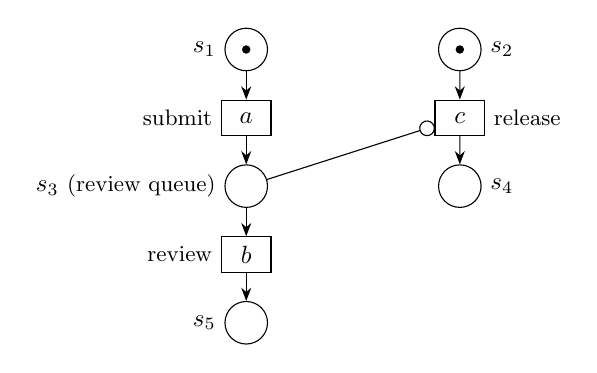
\begin{tikzpicture}[
  place/.style={circle,draw,minimum size=6mm,inner sep=0pt},
  trans/.style={rectangle,draw,minimum width=7mm,minimum height=5mm,inner sep=1pt},
  tok/.style={circle,fill,inner sep=1.2pt},
  >=Stealth, node distance=4mm, scale=0.9, transform shape]
  \node[place,label=left:{$s_1$}] (s1) {}; \node[tok] at (s1) {};
  \node[trans,below=of s1,label=left:{\small submit}] (a) {$a$};
  \node[place,below=of a,label=left:{$s_3$\ \small(review queue)}] (s3) {};
  \node[trans,below=of s3,label=left:{\small review}] (b) {$b$};
  \node[place,below=of b,label=left:{$s_5$}] (s5) {};
  \node[place,right=24mm of s1,label=right:{$s_2$}] (s2) {}; \node[tok] at (s2) {};
  \node[trans,below=of s2,label=right:{\small release}] (c) {$c$};
  \node[place,below=of c,label=right:{$s_4$}] (s4) {};
  \draw[->] (s1) -- (a); \draw[->] (a) -- (s3); \draw[->] (s3) -- (b); \draw[->] (b) -- (s5);
  \draw[->] (s2) -- (c); \draw[->] (c) -- (s4);
  \draw[-{Circle[open,length=2mm]}] (s3) -- (c);
\end{tikzpicture}
\caption{The review and release net, an elementary net with an inhibitor arc (ending in a circle): a change is submitted to the review queue $s_3$ and reviewed, and a release $c$ may begin only while the queue is empty. It is the net of Fig.~5.1 in~\cite{Alqarni2016} and of Sect.~6 in~\cite{AlqarniJanicki2018}.}
\label{fig:net}
\end{figure}

\begin{example}[Review and release]
\label{ex:fig1}
Figure~\ref{fig:net} shows the running example of our earlier work. Read as an at-start system (Section~\ref{sec:nets} gives the translation), its states are markings, $a$ needs $s_1$, $b$ needs $s_3$, $c$ needs $s_2$ and an empty $s_3$, and $b, c$ are independent. Under the consuming discipline, from $\{s_2, s_3\}$ the action $b$ is enabled, $c$ is not, and after $\B{b}$ the action $c$ is enabled: the review takes the change off the queue when it begins and the release finds the queue empty. The word $\B{a}\,\E{a}\,\B{b}\,\B{c}\,\E{c}\,\E{b}$ is a complete run from $\{s_1, s_2\}$ although $\{a\}\{b, c\}$ is not a step sequence. Under the committed discipline, from $\{s_1, s_2\}$ the complete runs in which $a, b, c$ each occur once are exactly the ten interval firing sequences listed in~\cite[Sect.~7]{AlqarniJanicki2018},
\[
\begin{array}{ll}
\B{a}\E{a}\B{b}\E{b}\B{c}\E{c} & \B{c}\E{c}\B{a}\E{a}\B{b}\E{b}\\
\B{a}\B{c}\E{c}\E{a}\B{b}\E{b} & \B{a}\B{c}\E{a}\E{c}\B{b}\E{b}\\
\B{c}\B{a}\E{c}\E{a}\B{b}\E{b} & \B{c}\B{a}\E{a}\E{c}\B{b}\E{b}\\
\B{a}\B{c}\E{a}\B{b}\E{b}\E{c} & \B{a}\B{c}\E{a}\B{b}\E{c}\E{b}\\
\B{c}\B{a}\E{a}\B{b}\E{b}\E{c} & \B{c}\B{a}\E{a}\B{b}\E{c}\E{b}
\end{array}
\]
and the consuming discipline yields these ten and exactly two more,
\[
\B{a}\E{a}\B{b}\B{c}\E{c}\E{b} \qquad\text{and}\qquad \B{a}\E{a}\B{b}\B{c}\E{b}\E{c},
\]
in both of which review and release overlap. Both counts are verified by complete enumeration in Lean (Section~\ref{sec:lean}).
\end{example}

The example also shows a run the committed discipline does allow: in $\B{c}\,\B{a}\,\E{a}\,\B{b}\,\E{b}\,\E{c}$ the release begins while the queue is empty, and a change is submitted and reviewed before the release ends. Its interval order is consistent with an observation in which the release takes effect before the submission, which is why the interval reading accepts it. Whether the policy of the system accepts it is a separate question, and the answer is a condition that must hold \emph{throughout} the release. That is the subject of Part~B.

% =====================================================================
\section{Part B: Conditions Throughout and at the End}
\label{sec:partB}

With over-all and end conditions, blocks of actions stop being the right unit of comparison. In a block all beginnings precede all endings, so a block never shows what an ending does to the over-all condition of another action in flight, and a block from a state never shows what happens to actions that were in flight already. Two decisions follow. We start from coherent configurations, and we compare the interval semantics with homogeneous event steps.

\begin{remark}[Why configurations]
\label{rem:states}
Starting only from states with nothing in flight, the two-action conditions below are sufficient but not necessary. There is a committed system with three actions $a, b, c$, all independent, in which every pair and every state passes every two-action condition, yet the block word $\B{a}\,\B{b}\,\B{c}\,\E{b}\,\E{c}\,\E{a}$ from a state where all three are enabled is not a run: the over-all condition of $a$ is $\neg(x \wedge y)$, the endings of $b$ and $c$ set $x$ and $y$, the start condition of $a$ is $\neg y$ and that of $c$ is $\neg x$, so the state $(x, y) = (1, 0)$ with $a$ in flight, at which $c$'s ending does the damage, can be reached only inside a block of size three. From coherent configurations the same state is a legitimate start, with $a$ in flight, and the two-action condition catches it. The configuration convention is also the one under which the net constructions of Section~\ref{sec:nets} are literally instances, since there every marking is a configuration.
\end{remark}

\subsection{Homogeneous steps and event transparency}

\begin{definition}[Homogeneous step conservativity]
\label{def:hsc}
$\D$ is \emph{homogeneous-step conservative} if for every coherent configuration $c$, every nonempty set $U$ of pairwise independent actions and every configuration $c'$, the following are equivalent, and likewise with endings in place of beginnings:
(1) $U$ is a beginning step at $c$ and firing it leads to $c'$;
(2) every order of the beginnings of $U$ runs from $c$ to $c'$;
(3) some order of the beginnings of $U$ runs from $c$ to $c'$.
\end{definition}

For an at-start system a block word is a beginning step followed by an ending step, and Proposition~\ref{prop:bridge} shows that homogeneous step conservativity is then step-conservativity. In general, homogeneous step conservativity says exactly when Janicki's interval step semantics~\cite{Janicki2019}, in which sets of beginnings or sets of endings fire a~priori, agrees with the plain interval semantics of sequences.

\begin{definition}[Event transparency]
\label{def:et}
$\D$ has \emph{transparent beginnings} if for every coherent configuration $c$, all independent $a, b$ and $\enB{a}{c}$,
\[
\enB{b}{c} \iff \enB{b}{c_a} \qquad\text{where } c \istep{\B{a}} c_a ,
\]
and \emph{transparent endings} if for every coherent $c$, all $a \neq b$ and $\enE{a}{c}$,
\[
\enE{b}{c} \iff \enE{b}{c^a} \qquad\text{where } c \istep{\E{a}} c^a .
\]
The \emph{forward half} of each condition is the implication from left to right (an event never disables another), the \emph{backward half} the implication from right to left (an event never enables another).
\end{definition}

The mixed pairs, a beginning against an ending, are deliberately not constrained. Their interference is legitimate: when the ending of $a$ enables the beginning of $b$, the history has $a \prec b$; when the ending of $a$ disables it, $b \wprec a$. These are the relations of interval order semantics, and a condition that excluded them would exclude every causal dependency between independent actions.

\begin{theorem}[Characterisation]
\label{thm:B-char}
Let $\D$ be a durative guarded action system.
\begin{enumerate}
\item[(i)] Every enabled homogeneous step runs in every order, (1)$\Rightarrow$(2) in Definition~\ref{def:hsc}, if and only if the forward halves of event transparency hold.
\item[(ii)] Every run of a homogeneous word is an enabled step, (3)$\Rightarrow$(1), if and only if the backward halves hold.
\item[(iii)] Consequently $\D$ is homogeneous-step conservative if and only if its beginnings and its endings are transparent.
\end{enumerate}
\end{theorem}

\begin{proof}
(i) Sufficiency: let $U$ be a beginning step at the coherent $c = (t, F)$ and $b_1 \cdots b_k$ an order of $U$. $\B{b_1}$ is enabled at $c$ and leads to a coherent configuration $c_1$; for every later $b_i$, independent of $b_1$, the forward half gives $\enB{b_i}{c_1}$, so the rest of $U$ is a beginning step at $c_1$, and induction on $k$ finishes, the final configuration being $(\acq_U(t), F \cup U)$ by commutation. Endings are the same with the release parts and $F \setminus U$. Necessity: if $a, b$ are independent and both enabled at $c$, then $\{a, b\}$ is a beginning step, so $\B{a}\,\B{b}$ runs, so $\B{b}$ is enabled after $\B{a}$; and similarly for endings, where $a, b \in F$ are independent by coherence.

(ii) Sufficiency: if $\B{b_1} \cdots \B{b_k}$ runs from $c$, then $\B{b_1}$ is enabled at $c$, and by induction the remaining beginnings form a beginning step at $c_1$; each $b_i$ is independent of $b_1$ because its beginning was enabled with $b_1$ in flight, and the backward half brings its enabledness back from $c_1$ to $c$. Endings likewise. Necessity: if $\B{a}$ is enabled at $c$ and $\B{b}$ after it, then $\B{a}\,\B{b}$ runs, so by (3)$\Rightarrow$(1) the set $\{a, b\}$ is a beginning step at $c$, so $\B{b}$ is enabled at $c$.

(iii) Conservativity is the conjunction of (1)$\Rightarrow$(2) and (3)$\Rightarrow$(1), since (2)$\Rightarrow$(3) always holds for nonempty $U$.
\end{proof}

\begin{theorem}[Soundness]
\label{thm:B-sound}
$\D$ is Janicki-sound if and only if, at every coherent configuration, whenever $\B{a}\,\B{b}$ runs so does $\B{b}\,\B{a}$, and whenever $\E{a}\,\E{b}$ runs so does $\E{b}\,\E{a}$. Homogeneous step conservativity implies Janicki-soundness, and not conversely.
\end{theorem}

\begin{proof}
A swap inside a run happens at the configuration reached so far, which is coherent, and both orders of the two events lead to the same configuration by commutation; so closure at every coherent configuration for two-event runs is closure for all runs. If beginnings are transparent and $\B{a}\,\B{b}$ runs from $c$, then $\B{b}$ is enabled at $c$ by the backward half and $\B{a}$ after it by the forward half; endings likewise. Example~\ref{ex:sound-not-transparent} separates the two notions.
\end{proof}

\begin{proposition}[At-start systems]
\label{prop:bridge}
For an at-start system, transparent beginnings is acquire-transparency, endings are always transparent, homogeneous step conservativity is step-conservativity, and Janicki-soundness is the swap condition.
\end{proposition}

\begin{proof}
With $\ovr_b = \stp_b = S$ the beginning of $b$ is enabled at $(t, F)$ iff $b \notin F$, $b$ conflicts with nothing in $F$ and $t \in \en_b$; the first two conjuncts are unchanged by the beginning of an action independent of $b$, so transparent beginnings reduces to $t \in \en_b \iff \acq_a(t) \in \en_b$ for $t \in \en_a$, and the configuration $(t, \emptyset)$ shows the reduction is exact. The ending of $b$ is enabled iff $b \in F$, which the ending of $a \neq b$ does not change. The remaining equivalences then follow from Theorems~\ref{thm:A-char}, \ref{thm:A-sound}, \ref{thm:B-char} and~\ref{thm:B-sound}.
\end{proof}

\subsection{What the conditions say about the three readings}

Event transparency is a condition on enabledness, and enabledness is a conjunction of conditions on several condition sets. Unfolding it gives readable sufficient clauses, one per condition set and per part of an effect; they are the clauses one would first write down, and they are not necessary in general, because a clause may fail at a state where the event it speaks about is blocked for another reason. In pure cases they are exact. We give the two that matter most.

\begin{theorem}[Committed discipline]
\label{thm:committed-BB}
Under the committed discipline beginnings are transparent, whatever the conditions.
\end{theorem}

\begin{proof}
With $\acq_a = \id$, the beginning of $a$ changes only the in-flight set, by adding $a$. For $b$ independent of $a$ the conjuncts $b \notin F$ and ``$b$ conflicts with nothing in $F$'' are unaffected, and the new conjunct $\acq_b(t) \in \ovr_a$ holds because $\enB{a}{c}$ includes $\acq_a(t) = t \in \ovr_a$ and $\acq_b(t) = t$.
\end{proof}

So under the committed discipline only endings can misbehave, and they do so through over-all and end conditions. The over-all case is the one of locks and read arcs.

\begin{definition}[Lock condition]
\label{def:lock}
$\D$ satisfies the \emph{lock condition} if for all independent $a, b$ and every state $t \in \ovr_a \cap \ovr_b \cap \stp_b$, $\rel_b(t) \in \ovr_a$: the ending of an action never falsifies the over-all condition of an independent action in flight.
\end{definition}

\begin{theorem}[Lock theorem]
\label{thm:lock}
Let $\D$ have the committed discipline and no end conditions ($\stp_a = S$ for all $a$).
\begin{enumerate}
\item[(i)] If $\D$ satisfies the lock condition, its endings are transparent, and $\D$ is homogeneous-step conservative and Janicki-sound.
\item[(ii)] At a configuration with exactly two actions $a, b$ in flight, endings are transparent in both orders if and only if $\rel_a(t) \in \ovr_b \iff \rel_b(t) \in \ovr_a$: either ending falsifies the other's over-all condition, or neither does.
\item[(iii)] Let $a, b$ \emph{interfere} if some $t \in \ovr_a \cap \ovr_b$ has $\rel_b(t) \notin \ovr_a$ or $\rel_a(t) \notin \ovr_b$. The system obtained by adding a conflict on every interfering pair satisfies the lock condition, and is therefore homogeneous-step conservative.
\end{enumerate}
\end{theorem}

\begin{proof}
(i) Let $c = (t, F)$ be coherent, $a \neq b$ in $F$, $\enE{a}{c}$. The ending of $b$ is enabled at $c$ iff $\rel_b(t) \in \ovr_d$ for all $d \in F \setminus \{b\}$, and at $c^a = (\rel_a(t), F \setminus \{a\})$ iff $\rel_b(\rel_a(t)) \in \ovr_d$ for all $d \in F \setminus \{a, b\}$. By the lock condition at $t$, where every $d \in F$ is in flight and coherent, the first holds; by the lock condition at $\rel_a(t)$, which is coherent for $F \setminus \{a\}$ because $\E{a}$ was enabled, the second holds. (ii) With $F = \{a, b\}$ and no end conditions, $\enE{a}{c}$ is $\rel_a(t) \in \ovr_b$, $\enE{b}{c}$ is $\rel_b(t) \in \ovr_a$, and after either ending the other is enabled unconditionally; so the two clauses of transparency are the two implications. (iii) In the new system independent pairs do not interfere, which is the lock condition; the commutation requirements only weaken when conflicts are added.
\end{proof}

With three actions in flight the lock condition is still sufficient but the exact condition is transparent endings itself; the interference may involve a third action's over-all condition that only the joint effect of two endings falsifies. Theorem~\ref{thm:lock}(iii) is a repair, not in general the least one. By (ii), a pair whose interference is asymmetric at some state must be in conflict in every extension with transparent endings, but a pair whose two endings always falsify each other's condition blocks itself, and the following example shows that no least repair need exist at all.

\begin{remark}[No least repair in Part B]
\label{rem:noleast}
Take three independent committed actions on a counter $n \in \{0, 1, 2\}$, each requiring $n \le 1$ at its start and over all, with no end condition, and each incrementing $n$ when it ends, capped at $2$. With all three in flight at $n = 0$ every ending is enabled, but after one ending $n = 1$ and any further ending would set $n = 2$ while an action is still in flight; so endings are not transparent and the system is not homogeneous-step conservative. Adding any single conflict, between $a$ and $b$, or $a$ and $c$, or $b$ and $c$, removes the configurations with three actions in flight, and with at most two in flight the endings are transparent: at $n = 0$ both run in either order, at $n = 1$ both are blocked. The three repairs are incomparable and their intersection, the original system, is not conservative. Theorem~\ref{thm:lock}(iii) adds all three conflicts. The example is mechanised (\lean{Three.nlr0\_not\_hsc}, \lean{Three.nlrAB\_hsc} and its two companions). It was found by a referee of an earlier version.
\end{remark}

\subsection{The classification}
\label{sec:cells}

The conditions of an action may be read at its start, over all of it, or at its end, and its effects may be published at its end (committed), at its beginning (start-only), or at both ends (consuming, in the sense of consuming at the beginning and producing at the end). Precisely, a system is in the cell \emph{at start} when $\ovr_a = \stp_a = S$ for every action, in the cell \emph{over all} when $\st_a = \ovr_a$ and $\stp_a = S$, and in the cell \emph{at end} when $\st_a = \ovr_a = S$; it is \emph{committed} when $\acq_a = \id$, \emph{start-only} when $\rel_a = \id$, and otherwise has effects at both ends. (An over-all condition is also read at the start: it must hold in the state just after the beginning, and under the committed discipline that state is the state before it.) Table~\ref{tab:cells} classifies the nine combinations. In two of them every system is homogeneous-step conservative and sound; in each of the other seven there is a system with two actions that is not.

\begin{table}[t]
\centering
\caption{The nine combinations of condition placement and effect placement. ``All'' means that every system in the cell is homogeneous-step conservative and Janicki-sound (a theorem); a name $N$ is a two-action system in the cell that is neither, mechanised in Lean as the pair of theorems \lean{N\_not\_hsc} and \lean{N\_not\_jsound}, with the kind of interference that breaks it. The last column records whether a system in the cell may reach states by overlapping actions that it cannot reach sequentially (Section~\ref{sec:gap}).}
\label{tab:cells}
\footnotesize
\resizebox{\textwidth}{!}{%
\begin{tabular}{@{}lllll@{}}
\toprule
Effects & Conditions & Sound and consistent & Interference & Required concurrency \\
\midrule
end (committed) & at start & all (Cor.~\ref{cor:committed}) & none & possible \\
end & over all & \lean{committedOverall} & endings & impossible \\
end & at end & \lean{committedAtEnd} & endings & impossible \\
beginning (start-only) & at start & \lean{startOnlyAtStart} & beginnings & impossible \\
beginning & over all & \lean{startOnlyOverall} & beginnings & impossible \\
beginning & at end & all (Thm.~\ref{thm:cells}) & none & possible \\
both ends (consuming) & at start & \lean{consumingAtStart} & beginnings & possible \\
both ends & over all & \lean{consumingOverall} & beginnings & possible \\
both ends & at end & \lean{consumingAtEnd} & endings & possible \\
\bottomrule
\end{tabular}}
\end{table}

\begin{theorem}[The two sound cells]
\label{thm:cells}
\begin{enumerate}
\item[(i)] Every at-start system with the committed discipline is homogeneous-step conservative and Janicki-sound.
\item[(ii)] Every system with the start-only discipline and conditions read only at the end ($\st_a = \ovr_a = S$) is homogeneous-step conservative and Janicki-sound.
\item[(iii)] In each of the other seven combinations there is a system with two independent actions and one or two Boolean variables that is neither.
\end{enumerate}
\end{theorem}

\begin{proof}
(i) is Theorem~\ref{thm:committed-BB} together with Proposition~\ref{prop:bridge}. (ii) Without start and over-all conditions, the beginning of $b$ is enabled at $(t, F)$ iff $b \notin F$ and $b$ conflicts with nothing in $F$, which the beginning of an independent $a$ does not change; the ending of $b$ is enabled iff $b \in F$ and $t \in \stp_b$, and the ending of $a \neq b$ changes neither, since $\rel_a = \id$. (iii) The witnesses are the following, all with no conflicts. For each, Lean checks that the relevant transparency condition fails at some coherent configuration and that some two-event run cannot be swapped, so both properties fail.
\begin{itemize}
\item Committed, over all: $a$ and $b$ both require $p$ at their start and over all; $b$ clears $p$ when it ends. With both in flight, $\E{a}$ is enabled and $\E{b}$ is not, since it would falsify the over-all condition of $a$; after $\E{a}$ it is. So $\E{a}\,\E{b}$ runs while $\E{b}\,\E{a}$ does not. This is the revocation trace.
\item Committed, at end: $a$ requires $p$ at its end; $b$ clears $p$ when it ends. $\E{a}\,\E{b}$ runs and $\E{b}\,\E{a}$ does not.
\item Start-only, at start: $a$ requires $p$ at its start; $b$ clears $p$ when it begins. $\B{a}\,\B{b}$ runs and $\B{b}\,\B{a}$ does not (Example~\ref{ex:AN0}).
\item Start-only, over all: $a$ requires $p$ to be absent at its start and over all; $b$ clears $p$ when it begins. From $p$ present, $\B{b}\,\B{a}$ runs and $\B{a}$ cannot start first. (With $a$ requiring the presence of $p$ instead, as a referee of an earlier version pointed out, each beginning blocks the other and only conservativity fails.)
\item Consuming, at start: $a$ requires $p$ at its start; $b$ clears $p$ when it begins and sets $q$ when it ends. $\B{a}\,\B{b}$ runs and $\B{b}\,\B{a}$ does not.
\item Consuming, over all: $a$ requires $p$ absent at its start and over all; $b$ clears $p$ when it begins and sets $q$ when it ends. $\B{b}\,\B{a}$ runs and $\B{a}\,\B{b}$ does not.
\item Consuming, at end: $a$ requires $q$ false at its end; $b$ clears $p$ when it begins and sets $q$ when it ends. $\E{a}\,\E{b}$ runs and $\E{b}\,\E{a}$ does not.
\end{itemize}
\end{proof}

The two sound cells are mirror images of each other: in the first, endings may interfere with beginnings (the ending of $a$ may disable or enable the beginning of $b$, giving $b \wprec a$ or $a \prec b$), in the second, beginnings may interfere with endings. In both, every interaction between a condition of one action and an effect of another relates a beginning to an ending, which is exactly what precedence and weak precedence express; Section~\ref{sec:structures} shows that the interactions of the other cells, between two beginnings or two endings, fall outside that language.

The practical reading is this. When every condition is read at the start, soundness is a matter of discipline: publish effects at the end. When every condition is read at the end, the mirror choice works: publish effects at the beginning (Theorem~\ref{thm:cells}(ii)). Conditions that must hold throughout are made sound by no placement of effects: under each of the three disciplines some system with over-all conditions is not closed under swaps. What makes such a system sound is a conflict with every action whose effect can falsify the condition; Theorem~\ref{thm:lock}(iii) gives one choice of conflicts, and Remark~\ref{rem:noleast} shows that there need be no least one. Over-all conditions are locks, and no accounting of visibility replaces the lock.

% =====================================================================
\section{Temporal Gaps and Required Concurrency}
\label{sec:gap}

Cushing, Kambhampati, Mausam and Weld ask when temporal planning is really temporal, that is, when a problem has solutions only with overlapping actions~\cite{CushingEtAl2007}. Their answer is syntactic. An action has a \emph{temporal gap} when there is no single instant of its duration at which all its conditions and effects hold together; a sub-language of PDDL2.1 is \emph{temporally simple}, every solvable problem has a sequential solution, if and only if it forbids temporal gaps (their Theorem~6). We prove the per-system form of this result for arbitrary state spaces, and show that each way of having a gap can require concurrency.

\begin{definition}[Temporal gap]
\label{def:gap}
An action $a$ of $\D$ has \emph{no temporal gap} if either $\acq_a = \id$ and $\ovr_a \cap \stp_a \subseteq \st_a$ (all effects at the end, and the over-all and end conditions imply the start condition there), or $\rel_a = \id$ and $\acq_a(t) \in \stp_a$ whenever $t \in \st_a$ and $\acq_a(t) \in \ovr_a$ (all effects at the beginning, and the start and over-all conditions imply the end condition). The system has no temporal gap if no action has one.
\end{definition}

The definition is the semantic version of Cushing et al.'s: with effects at the end, a start condition that is not implied by the over-all condition is separated from the effect by a gap; with effects at the beginning, an end condition not implied by the over-all condition is. We take the implications at the states where they are needed rather than as inclusions of condition sets, which is slightly weaker than the syntactic criterion and is what the proof uses.

\begin{definition}[Two reachability relations]
A state $s'$ is \emph{interval-reachable} from $s$ if some complete run leads from $(s, \emptyset)$ to $(s', \emptyset)$. It is \emph{sequentially reachable} if it is reachable by complete runs of the form $\B{a_1}\,\E{a_1}\, \B{a_2}\,\E{a_2} \cdots$, in which no two actions overlap.
\end{definition}

Sequential reachability is the reachability of the step semantics restricted to singleton steps, with each action checked as it would be in isolation: $a$ fires from $t$ when $t \in \st_a$, $\acq_a(t) \in \ovr_a \cap \stp_a$, and leads to $\eff_a(t)$. Sequentially reachable states are interval-reachable.

\begin{theorem}[No gap, no required concurrency]
\label{thm:nogap}
If $\D$ has no temporal gap, then interval reachability and sequential reachability coincide.
\end{theorem}

\begin{proof}
We show that along every run from a coherent configuration the current state remains sequentially reachable from the initial state. Let $(t, F) \istep{e} (t', F')$ with $t$ sequentially reachable from $s$. If $e = \B{a}$ and $a$ has all effects at the end, then $t' = t$. If $e = \B{a}$ and $a$ has all effects at the beginning, then $t' = \acq_a(t)$; the beginning was enabled, so $t \in \st_a$ and $\acq_a(t) \in \ovr_a$, hence $\acq_a(t) \in \stp_a$ by the no-gap condition, and $a$ fires from $t$ to $\rel_a(\acq_a(t)) = t'$. If $e = \E{a}$ and $a$ has all effects at the beginning, then $t' = t$. If $e = \E{a}$ and $a$ has all effects at the end, then $t' = \rel_a(t)$; the ending was enabled, so $t \in \stp_a$, coherence gives $t \in \ovr_a$, the no-gap condition gives $t \in \st_a$, and $a$ fires from $t$ to $\rel_a(\acq_a(t)) = t'$. An action without effects at either end falls under the first case. A complete run ends at a state, which is therefore sequentially reachable.
\end{proof}

This is Cushing et al.'s rescheduling argument, the states between consecutive critical points being the same in the overlapping and in the sequential run, carried out as an invariant on configurations; there is nothing to reschedule, because every effect is applied at a point of the run at which the action could also have fired alone.

\begin{proposition}[Witnesses]
\label{prop:gap-witnesses}
Each way of having a temporal gap admits a system with two independent actions in which a state is interval-reachable but not sequentially reachable.
\begin{enumerate}
\item[(i)] Start conditions with effects at the end: $a$ requires $y$ false and sets $x$ when it ends, $b$ requires $x$ false and sets $y$ when it ends. From $(0, 0)$ the run $\B{a}\,\B{b}\,\E{a}\,\E{b}$ reaches $(1, 1)$; sequentially, whichever action fires first disables the other.
\item[(ii)] End conditions with effects at the beginning: $a$ sets $x$ when it begins and requires $y$ to end, $b$ sets $y$ when it begins and requires $x$ to end. From $(0, 0)$ the same run reaches $(1, 1)$; sequentially, neither action can end.
\item[(iii)] Effects at both ends: $a$ sets $x$ when it begins and clears it when it ends, $b$ requires $x$ at its start and sets $y$ when it ends. From $(0, 0)$ the run reaches $(0, 1)$; sequentially, $x$ is never set when $b$ is checked.
\end{enumerate}
\end{proposition}

The three witnesses are the abstract forms of Cushing et al.'s Figures~1(a), 1(b) and~1(d): mutual disabling by end effects, mutual enabling by start effects, and a condition that holds only during another action. The first is also the pattern of the net $N_{io}$ of~\cite{AlqarniJanicki2018}, which has neither firing sequences nor step sequences between two of its markings but does have an interval run, and of the strict-expressiveness theorem of the conference version of this work, which is a committed-discipline instance of the same known phenomenon. The three witnesses are mechanised: interval reachability by exhibiting the run, sequential unreachability by an inductive invariant.

\begin{corollary}[The table's last column]
\label{cor:table-gap}
In the cells committed/over all, committed/at end, start-only/at start and start-only/over all, no system has a temporal gap, so interval reachability is sequential reachability. In each of the other five cells there is a two-action system with required concurrency.
\end{corollary}

\begin{proof}
For a committed action $\ovr_a \cap \stp_a \subseteq \st_a$ holds when $\st_a = \ovr_a$ (over all) or $\st_a = S$ (at end); for a start-only action the end condition is $S$ in the cells at start and over all. Theorem~\ref{thm:nogap} gives the first claim. Proposition~\ref{prop:gap-witnesses} gives witnesses for committed/at start, start-only/at end and both ends/at start; reading the condition of $b$ in (iii) over all or at its end gives witnesses for the two remaining cells, mechanised under the names \lean{gapBothEndsOverall} and \lean{gapBothEndsAtEnd}.
\end{proof}

Table~\ref{tab:cells} now shows a correspondence that Theorems~\ref{thm:cells} and~\ref{thm:nogap} make exact. Among the six cells with effects at one end, the two in which every system is sound and consistent, conditions at the start with effects at the end and conditions at the end with effects at the beginning, are precisely the two in which an action can have a temporal gap; in the other four, interval reachability is sequential reachability. The cells with effects at both ends admit gaps but are not sound. (Under the system-wide definition of the cells a both-ends system may have no gap at all, for instance one start-only and one committed action without conditions; the entry ``possible'' is an existence claim.) So among the disciplines that publish at one end, interval orders are a safe abstraction of the runs exactly where the interval semantics also reaches states that no sequence of non-overlapping actions reaches: the semantics is faithful where it is indispensable, and where it adds nothing to reachability it is also where it can mislead.

% =====================================================================
\section{Histories and Their Structures}
\label{sec:structures}

A concurrent history is a set of runs that are the same up to the order of independent events. For the interval semantics of inhibitor nets, histories are the runs of one process, and they are described by relational structures carrying precedence and weak precedence~\cite{JanickiKoutny1993,AlqarniJanicki2018,JanickiKleijnKoutnyMikulski2024}: the history is the set of interval orders that extend its invariant structure. We ask whether this remains true under the other combinations of the table. The abstract model has no processes, so we first need a notion of history, and the choice matters.

\begin{definition}[Histories, representability]
\label{def:history}
Let $X \subseteq A$ and let $c_0, c_1$ be configurations. The \emph{end-point history} $H(X, c_0, c_1)$ is the set of complete words over $X$ that run from $c_0$ to $c_1$. Two words of it are \emph{adjacent} if they differ by swapping two neighbouring events of distinct actions; a \emph{history} is a connected component of an end-point history under adjacency, that is, a class of runs that can be transformed into one another by swaps of adjacent events both of whose orders are runs with the same end points. For a set $H$ of complete words over $X$, its set of interval orders is $\IO(H) = \{\prec_w \mid w \in H\}$, and its invariant structure consists of the precedences common to all its words and the pairs $(a, b)$ with $b \prec_w a$ in no word of $H$ (weak precedence). An interval order on $X$ \emph{extends} the invariant structure if it contains every common precedence and reverses no weak precedence; $H$ is \emph{representable} if $\IO(H)$ is exactly the set of interval orders extending its invariant structure, and \emph{closed} if every complete word over $X$ whose interval order is in $\IO(H)$ belongs to $H$.
\end{definition}

Histories in this sense are the abstract counterpart of processes: two runs are in the same history when they differ only in the order of events that could have happened in either order at that point. Closedness is soundness restricted to one history: by Theorem~\ref{thm:B-sound} a Janicki-sound system has only closed histories. Representability is the stronger statement that a single structure of precedence and weak precedence describes the history, as the interval order structures of~\cite{JanickiKoutny1993} and the invariant combined structures of~\cite{JanickiKleijnKoutnyMikulski2024} do for the processes of inhibitor nets~\cite{AlqarniJanicki2018}.

The distinction between end-point histories and histories is not a technicality, and the review and release net shows it.

\begin{example}[Why end points are not enough]
\label{ex:fig1-history}
Consider Fig.~\ref{fig:net} under the committed discipline, with the ten runs of Example~\ref{ex:fig1} as the end-point history from $\{s_1, s_2\}$ to $\{s_4, s_5\}$. The serial orders $c, a, b$ (release first, the queue being empty) and $a, b, c$ (release after the review has emptied the queue) are both runs, so no precedence or weak precedence fixes $c$ relative to $a$ or $b$; the invariant structure is $a \prec b$ alone. The serial order $a, c, b$ extends it but is not a run: when the release would begin, the submitted change is still in the queue. The ten runs realise four interval orders while six extend the invariant structure. So the end-point history is not representable, although the net is sound and consistent (Corollary~\ref{cor:committed}), and although Theorem~5 of~\cite{AlqarniJanicki2018} shows every process of such a net to be representable. The reason is that one absence test succeeds for two different reasons, an initially empty queue or a queue emptied by the review, and the end-point history merges the two. Under Definition~\ref{def:history} the ten runs fall into two histories: the single run $\B{a}\E{a}\B{b}\E{b}\B{c}\E{c}$, which no swap connects to the others since the release cannot begin while the review is in flight, and the nine remaining runs; both are representable. They correspond to the two processes of the net: in one the test of $s_3$ reads the initial condition, in the other the condition left by the review. All of this is checked in Lean (\lean{Three.fig1\_not\_representable}, \lean{Three.fig1\_two\_classes}). A referee of an earlier version found the example.
\end{example}

The propositions below exhibit non-representable histories. In each of them the end-point history is a single history under Definition~\ref{def:history}, which Lean verifies by computing the swap class, so the two notions agree there and the obstruction is not an artefact of merged processes.

\begin{proposition}[A constraint between beginnings]
\label{prop:beginbegin}
Let $t_0, t_1, t_2$ be independent actions under a consuming discipline on places $p, q$: $t_0$ requires $p$ and $q$ at its start and consumes both when it begins; $t_1$ requires $p$ at its start; $t_2$ requires $q$ empty at its start; no other conditions or effects. From $p, q$ marked, the end-point history over $\{t_0, t_1, t_2\}$ consists of $15$ complete runs, is a single history, and is not representable.
\end{proposition}

\begin{proof}
The run set forces $\B{t_1}$ before $\B{t_0}$, since $t_1$ needs the token that $t_0$ removes at its beginning, and $\B{t_0}$ before $\B{t_2}$, since $t_2$ needs $q$ empty. Both constraints are between beginnings. The invariant structure has no precedence and the weak precedences $t_0 \wprec t_2$, $t_1 \wprec t_0$, $t_1 \wprec t_2$; the interval order with $t_1 \prec t_0$ and all other pairs incomparable extends it, but no run realises it: $t_1 \prec t_0$ places $\E{t_1}$ before $\B{t_0}$, hence before $\B{t_2}$, so $t_1 \prec t_2$ as well. The enumeration of all $90$ complete words and the comparison of the two sets are carried out in Lean.
\end{proof}

\begin{proposition}[A constraint between endings]
\label{prop:endend}
Let $a, b, c$ be independent actions under the committed discipline on one place $p$: $a$ requires $p$ at its start and over all; $b$ requires $p$ at its start and consumes it when it ends; $c$ has no conditions and no effects. From $p$ marked, the end-point history over $\{a, b, c\}$ consists of $45$ complete runs, is a single history, and is not representable. The history over $\{a, b\}$ alone has three runs and is representable but not closed.
\end{proposition}

\begin{proof}
With $a$ and $b$ both in flight, $\E{b}$ would falsify the over-all condition of $a$, so $\E{a}$ precedes $\E{b}$ in every run in which both are in flight at some point, and $a$ cannot begin after $b$ has ended because $p$ is gone; the constraint is between two endings. For two actions the history has three runs and, by inspection, excludes only $b \prec a$, so $\IO(H)$ is the set of extensions of $a \wprec b$; but the word $\B{a}\,\B{b}\,\E{b}\,\E{a}$, with the same interval order as the run $\B{a}\,\B{b}\,\E{a}\,\E{b}$, is not a run. With the third action, $b \prec c$ together with $\E{a}$ before $\E{b}$ forces $a \prec c$; the interval order with $b \prec c$ and $a$ overlapping both extends the invariant structure and no run realises it. Again the sets are compared by enumeration in Lean.
\end{proof}

The two propositions answer a question left open by the recent structural theory: which features of a system produce histories within the framework of precedence and weak precedence. A reading at the start under the committed discipline relates every condition to the end of the action that writes what it reads; both constraints are between a beginning and an ending, and the processes of the inhibitor nets of~\cite{AlqarniJanicki2018} stay within the framework. The consuming discipline relates a condition read at the start to the beginning of the writer, and an over-all condition relates the end of the reader to the end of the writer. With two actions these constraints show as a loss of closedness; with a third action they propagate into conditional constraints that no single structure captures.

\begin{remark}[Representability also depends on the conditions]
\label{rem:disjunctive}
Soundness depends on the discipline and the placement of conditions; representability depends also on the language in which conditions are written. Consider three independent committed actions on Booleans $p, q, r$: $t_0$ requires $q$ or $r$ at its start and sets $p$ when it ends; $t_1$ clears $r$ when it ends; $t_2$ sets $q$ when it ends. The system is sound and consistent by Corollary~\ref{cor:committed}, but from $r$ marked the end-point history over the three actions, which has $81$ runs and is a single history under Definition~\ref{def:history}, is not representable: $t_0$ may begin because $r$ is still there, which requires $t_0 \wprec t_1$, or because $t_2$ has produced $q$, which requires $t_2 \prec t_0$, and the two reasons are connected by swaps because $t_0$ can also begin while both hold. Unlike in Example~\ref{ex:fig1-history}, the merger survives the passage to histories. In an elementary net the disjunction would be two transitions and the two reasons two processes; whether the histories of Definition~\ref{def:history} always coincide with the processes of~\cite{AlqarniJanicki2018} for nets with single-place tests we leave open. The claim is checked in Lean as well.
\end{remark}

% =====================================================================
\section{Nets and Plans as Instances}
\label{sec:nets}

\subsection{Elementary nets with inhibitor arcs}

An elementary net with inhibitor arcs~\cite{JanickiKoutny1995} has places $P$, transitions $T$, for each transition its input places ${}^\bullet t$, output places $t^\bullet$ and inhibitor places ${}^\circ t$, and markings $M \subseteq P$. Its \emph{at-start system} $\G_N$ has the markings as states, the transitions as actions,
\[
\en_t = \{ M \mid {}^\bullet t \subseteq M,\ (t^\bullet \setminus {}^\bullet t) \cap M = \emptyset,\ {}^\circ t \cap M = \emptyset \},\qquad
\eff_t(M) = (M \setminus {}^\bullet t) \cup t^\bullet ,
\]
and $t \conf u$ when $t \neq u$ share a place of ${}^\bullet t \cup t^\bullet$ and ${}^\bullet u \cup u^\bullet$. For independent transitions the effects act on disjoint sets of places and commute. The step semantics of $\G_N$ is the a~priori step semantics of the net. The \emph{consuming} discipline, $\acq_t(M) = M \setminus {}^\bullet t$ and $\rel_t(M) = M \cup t^\bullet$, is the naive interval translation; Example~\ref{ex:fig1} shows that it is not step-conservative. The \emph{committed} discipline is step-conservative by Corollary~\ref{cor:committed}.

The interval representation of~\cite{AlqarniJanicki2015,AlqarniJanicki2018} is a net transformation: each transition $t$ becomes a beginning $\B{t}$, an in-flight place $m_t$ and an ending $\E{t}$, where $\B{t}$ consumes ${}^\bullet t$ and marks $m_t$, $\E{t}$ unmarks $m_t$ and produces $t^\bullet$, and each inhibitor arc from $p$ to $u$ becomes two inhibitor arcs to $\B{u}$, one from $p$ and one from $m_r$ for every $r$ consuming from $p$. We read it as a system, the \emph{double-arc system} of $N$: its states are sets of places and markers, $\acq_t(M) = (M \setminus {}^\bullet t) \cup \{m_t\}$, $\rel_t(M) = (M \setminus \{m_t\}) \cup t^\bullet$, $\en_t$ additionally requires that no marker $m_r$ with ${}^\bullet r \cap {}^\circ t \neq \emptyset$ is present, and the conflict relation is that of $\G_N$. It changes the state space, so it is not a discipline for $\G_N$ in the sense of Definition~\ref{def:das}. It is, however, the committed discipline in disguise.

\begin{proposition}[The double arc is the committed discipline; paper proof]
\label{prop:double}
For a marking $M$ with markers let $\rho(M)$ be the marking of $N$ obtained by removing the markers and adding back ${}^\bullet r$ for every marker $m_r \in M$. Call a configuration $(M, F)$ of the double-arc system \emph{consistent} if the actions of $F$ are pairwise independent, $m_r \in M$ exactly when $r \in F$, and $M$ contains no place of ${}^\bullet r$ for $r \in F$; consistency holds for marker-free markings with $F = \emptyset$ and is preserved by every event. Then $(M, F) \mapsto (\rho(M), F)$ maps consistent configurations to configurations of $\G_N$ and commutes with every event: $\B{t}$ or $\E{t}$ is enabled at a consistent $(M, F)$ in the double-arc system if and only if it is enabled at $(\rho(M), F)$ in $\G_N$ under the committed discipline, and the successors correspond. In particular the two systems have the same runs from marker-free markings.
\end{proposition}

\begin{proof}
Endings are enabled in both systems exactly when $t \in F$, and $\rho(\rel_t(M)) = (\rho(M) \setminus {}^\bullet t) \cup t^\bullet = \eff_t(\rho(M))$: removing $m_t$ removes exactly the tokens ${}^\bullet t$ that $\rho$ had added back, $M$ itself contains none of them by consistency, and no other action in flight holds a place of ${}^\bullet t$ by independence. A beginning $\B{t}$ is blocked in both systems when $t \in F$ or $t$ conflicts with an action in flight, since both carry the same conflict relation. Otherwise the places that $\rho$ adds back are inputs of actions in $F$, all independent of $t$, hence disjoint from ${}^\bullet t \cup t^\bullet$, so ${}^\bullet t \subseteq M$ iff ${}^\bullet t \subseteq \rho(M)$ and $(t^\bullet \setminus {}^\bullet t) \cap M = \emptyset$ iff the same holds for $\rho(M)$; and ${}^\circ t \cap \rho(M) = \emptyset$ iff ${}^\circ t \cap M = \emptyset$ and no $r \in F$ has ${}^\bullet r \cap {}^\circ t \neq \emptyset$, which is exactly the double-arc guard. Finally $\rho(\acq_t(M)) = \rho(M)$, since the new marker $m_t$ adds back the places ${}^\bullet t$ that $\acq_t$ removed, matching $\acq_t = \id$ under the committed discipline; and the new configuration is consistent.
\end{proof}

So the double-arc construction is sound and step-consistent because it is committed for everything a guard can see: the second inhibitor arc is exactly what restores transparency after consuming the inputs at the beginning has broken it. For the net of Fig.~\ref{fig:net} the agreement of the two systems is also checked by enumeration in Lean.

The split net of~\cite{AlqarniJanicki2015,AlqarniJanicki2018} itself has no conflict relation; two transitions that share a place may overlap there whenever the tokens allow it, for instance a transition that consumes $p$ at its beginning and one that produces $p$ at its end. A referee of an earlier version exhibited a five-transition net, contact-free on all step-reachable markings, with such a run, which the double-arc system forbids. The two also differ on prefixes: the split net checks that an output place is empty when the transition ends, the double-arc system when it begins, so a transition whose output is marked may begin in the split net and then never end, while the double-arc system blocks it at once. On complete runs from a marking at which the net is contact-free, in which overlapping transitions are pairwise independent, neither difference arises, and the two agree; in particular they agree on all block words of steps, so Proposition~3 of~\cite{AlqarniJanicki2018}, the net form of Theorem~\ref{thm:A-char}, is the instance of that theorem for $\G_N$ under the committed discipline. A correspondence on all runs would need a system in which conflicting transitions may overlap, which Definition~\ref{def:das} does not provide, and we do not claim it.

\subsection{Activator nets and read arcs}

An activator (read) arc from $p$ to $t$ requires $p$ to be marked when $t$ fires and leaves it marked. Janicki's interval semantics of activator nets~\cite{Janicki2019} lets $\B{t}$ consume the inputs and test the activator places: a consuming discipline with a positive at-start condition. Example~\ref{ex:AN0} is his net $\mathit{AN}_0$, and his net $\mathit{AN}_2$, in which a step fires but no interval sequence of it does, is a failure of the forward half of transparency. The split construction of Chatain, Haar, Koutny and Schwoon~\cite{ChatainHaarKoutnySchwoon2015} keeps two copies of each place, a consumable copy taken by $t^-$ and a readable copy taken by $t^+$, so that a token stays readable until its consumer ends and a produced token appears, in both copies, when its producer ends; for the conditions of independent transitions this is the committed discipline, and the read arc is tested at $t^-$ only, so it is an at-start condition. Under it activator nets are sound and consistent by Corollary~\ref{cor:committed}, and plain interval sequences suffice, without the interval step sequences that~\cite{Janicki2019} introduces to restore consistency. The two constructions for read arcs differ exactly in the visibility discipline, and the asymmetry between inhibitor and activator nets observed in~\cite{Janicki2019} is the difference between the committed and the consuming discipline. Footnote~2 of that paper observes that for inhibitor nets the beginnings of a step can be fired in any order while for activator nets they cannot: that is the forward half of transparency.

If a read arc is instead meant as an over-all condition, the token must stay until the reader ends, and the consumer must wait. This is the cell ``committed, over all'' of Table~\ref{tab:cells}: the reader and the consumer interfere through their endings, and the system is sound only if they are declared in conflict, which is the asymmetric conflict of contextual nets~\cite{MontanariRossi1995,BaldanCorradiniMontanari2001} made symmetric. Theorem~\ref{thm:lock} gives the repair.

\subsection{PDDL2.1 durative actions}

A durative action of PDDL2.1~\cite{FoxLong2003} has conditions at start, at end and over all, and effects at start and at end, and a plan is a timed schedule. Our model is untimed, and the comparison has to respect that. Consider the fragment of durative actions with propositional conditions, unconditional propositional effects (literals added and deleted at each end), no numeric fluents, and unconstrained durations. Read a set of such actions as a system of Definition~\ref{def:das}: states are valuations, $\st_a$, $\ovr_a$ and $\stp_a$ are the three condition sets, $\acq_a$ applies the start effects and $\rel_a$ the end effects, and two actions conflict when they write a common proposition, so that the effects of independent actions commute. Goals aside, the runs of this system that start and finish with nothing in flight and the valid plans of the fragment correspond as follows. Every such run is the sequence of end points of a valid plan: give the events increasing times, which the free durations allow. The at-start and at-end conditions are checked in the same states by both semantics, and the open-interval reading of an over-all condition in~\cite{FoxLong2003} is the requirement that it hold after the beginning of its own action and after every event of another action while that action is in flight, which is Definition~\ref{def:interval}; the no-moving-targets rule of~\cite[Def.~12]{FoxLong2003} concerns simultaneous end points and is vacuous here. Conversely, a valid plan of the fragment whose end points are pairwise distinct, in which no action overlaps another instance of itself, and in which two actions that write a common proposition never overlap, is read as such a run by the same comparison. The three conditions on the plan are where the models differ. PDDL2.1 lets two overlapping actions write the same proposition at distinct instants, and it lets end points coincide subject to a rule checked per happening, where we have a static conflict relation; our model has at most one instance of an action in flight; and durations decide which sequences of end points a timed plan can realise, which our model ignores. Conditional effects whose condition is read at the start and whose effect is applied at the end are outside the fragment, since $\rel_a$ sees only the state at the end. Within the fragment, Theorem~\ref{thm:nogap} is the statement, for one set of actions rather than for a language, that without temporal gaps every state reached by a plan is reached by a sequential one, and Table~\ref{tab:cells} says which placements of conditions and effects have interval semantics that step semantics can safely stand in for. A referee of an earlier version pointed out the restrictions.

What our results add to the planning view is the soundness question. Plan validity is checked per plan. Event transparency is checked per system, and it says when the set of valid plans of the fragment is determined by the interval orders of the plans, so that a planner that reasons about interval orders rather than schedules, or a monitor that observes only the relative order of end points, loses nothing.

% =====================================================================
\section{Reading the Results for Tool-Using Agents}
\label{sec:agents}

Software agents that act through tool calls on a shared environment are a current source of long, overlapping, guarded actions: a call is issued, runs and returns, several calls may be in flight, and an action that needs a human approval may stay in flight for hours. The model applies as follows. A tool call is an action, issued at its beginning and taking effect at its end; the conflict relation is its footprint, the resources it writes or locks, as in the concurrency control of CoAgent~\cite{LyuEtAl2026CoAgent}, which models long transactions with prepare, execute and reverse phases; and the visibility discipline is a property of the platform, namely whether a call that takes a task from a queue, claims a ticket or moves an item to an in-progress state makes the change visible immediately or on completion.

Two examples of this paper mark the boundary of what each result guarantees.

\paragraph{The queue}
Example~\ref{ex:fig1}: a release may start only while no change is under review, the review takes the change off the queue when it begins, and the release starts during the review. The condition of the release is read at its start, and it is misled by a visible acquisition. Theorem~\ref{thm:A-char} says that this failure is exactly a failure of acquire-transparency, that the committed discipline removes it for every system, and that otherwise the least set of conflicts to add is the set of opaque pairs. This is the failure that a visibility discipline can prevent.

\paragraph{The revocation}
The cell ``committed, over all'' of Table~\ref{tab:cells}: a deployment requires an approval, the approval is revoked while the deployment is in flight, and the deployment takes effect. If the approval is read at the start of the deployment, every discipline permits this run, because nothing a beginning does to the state is at issue; the run is transparent, conservative and sound. The policy that is violated is that the approval hold \emph{throughout} the deployment, or at the instant its effect takes place. Writing it as an over-all condition changes the semantics in a precise way. Under the blocking reading the policy is enforced by construction: the revocation cannot end while the deployment is in flight, even with an empty conflict relation. What is lost is agreement with steps and the safety of the interval-order abstraction: the two endings interfere, and Theorem~\ref{thm:cells} says that no visibility discipline removes this for all systems. Theorem~\ref{thm:lock} says what does: a conflict between the deployment and every action that can revoke the approval, which also forbids the overlap outright, a stronger policy than the condition itself. The one cell with conditions after the start that is sound for every system is Theorem~\ref{thm:cells}(ii), conditions read at the end of actions whose effects are all at the beginning, which does not fit a deployment whose effect is what the approval is for. Under the validation reading, which is the situation of a platform that cannot block an external actor, the violation is detected rather than prevented, and what follows is an abort or a compensation, as in the saga-style mechanisms of~\cite{ChangGeng2025SagaLLM} and the reverse phase of~\cite{LyuEtAl2026CoAgent}; checking the approval again at the instant of the effect is then an implementation requirement that the model records as an at-end condition.

The empirical study of Lilienthal and Hong~\cite{LilienthalHong2025} describes time-of-check to time-of-use vulnerabilities in agents in which a value checked in one tool call is trusted by a later call after the environment may have changed; of the $66$ tasks of their benchmark, $56$ are labelled potentially vulnerable. Both of our examples are of this kind, and the two theorems say which of them a discipline can prevent and which only a conflict can. We make no claim that any particular platform follows one discipline or the other; the point of the results is that the question is well posed and decidable for a finite model of the platform's calls, their footprints, and the state their conditions read.

% =====================================================================
\section{Mechanisation in Lean 4}
\label{sec:lean}

The development is about $3{,}000$ lines of Lean~4~\cite{deMouraUllrich2021} over Mathlib~\cite{Mathlib2020}, toolchain \texttt{leanprover/lean4:v4.36.0-rc2} with Mathlib at tag \texttt{v4.36.0-rc2}; it builds with \texttt{lake exe cache get} followed by \texttt{lake build}. It contains no \texttt{sorry} and no \texttt{native\_decide}; every theorem depends only on the standard axioms of Lean (propositional extensionality, quotient soundness and choice), as reported by \texttt{\#print axioms}. The repository and its version are given at the end of the paper. Table~\ref{tab:lean} maps the statements of the paper to their formal counterparts.

A durative system is a structure with the commutation requirements as fields:

\begin{lstlisting}
structure DAS (S A : Type) where
  start : A → S → Prop
  over  : A → S → Prop
  stop  : A → S → Prop        -- the at-end condition
  acq : A → S → S
  rel : A → S → S
  conflict : A → A → Prop
  conflict_symm : ∀ a b, conflict a b → conflict b a
  acq_acq : ∀ a b, a ≠ b → ¬ conflict a b →
            ∀ s, acq a (acq b s) = acq b (acq a s)
  rel_rel : ∀ a b, a ≠ b → ¬ conflict a b →
            ∀ s, rel a (rel b s) = rel b (rel a s)
  acq_rel : ∀ a b, a ≠ b → ¬ conflict a b →
            ∀ s, acq a (rel b s) = rel b (acq a s)
\end{lstlisting}

\noindent Configurations are pairs of a state and a \texttt{Finset} of actions, so that the result of a step does not depend on the order of its events. Homogeneous steps are duplicate-free lists of pairwise independent actions, and the orders of a step are the permutations of the list. The at-start development of Part~A is kept as a separate structure \texttt{GAS}, with the conditions as two fields \texttt{pre} and \texttt{grd} whose conjunction is $\en$, and Proposition~\ref{prop:bridge} is the theorem that embeds it into \texttt{DAS}.

\begin{table}[t]
\centering
\caption{Statements of the paper and their formal counterparts. ``General'' means proved for all systems; ``kernel'' means a finite system checked by complete evaluation with \texttt{decide}; ``invariant'' means an inductive invariant.}
\label{tab:lean}
\footnotesize
\resizebox{\textwidth}{!}{%
\begin{tabular}{@{}lll@{}}
\toprule
Paper & Lean name & Kind \\
\midrule
Theorem~\ref{thm:A-char} & \lean{GAS.transparent\_iff\_conservative} & general \\
Theorem~\ref{thm:A-sound} & \lean{GAS.toDAS\_jsound\_iff}, \lean{GAS.transparent\_swapCond} & general \\
Example~\ref{ex:sound-not-transparent} & \lean{SoundNotTransparent.swapCond}, \lean{.not\_transparent} & kernel \\
Corollary~\ref{cor:A-repair} & \lean{GAS.repair\_conservative}, \lean{GAS.repair\_least} & general \\
Corollary~\ref{cor:A-swaprepair} & \lean{GAS.swapRepair\_jsound}, \lean{GAS.swapRepair\_least} & general \\
Corollary~\ref{cor:committed} & \lean{GAS.committed\_conservative}, \lean{DAS.committed\_atStart\_hsc} & general \\
Example~\ref{ex:fig1} & \lean{Fig1.committed\_runs\_eq\_thesis}, \lean{Fig1.consuming\_runs}, & kernel \\
 & \lean{Fig1.consuming\_not\_transparent}, \lean{Fig1.doubleArc\_runs\_eq\_thesis} & \\
Theorem~\ref{thm:B-char} & \lean{DAS.hsc\_fwd\_iff}, \lean{DAS.hsc\_bwd\_iff}, \lean{DAS.hsc\_iff\_et} & general \\
Theorem~\ref{thm:B-sound} & \lean{DAS.jsound\_iff}, \lean{DAS.hsc\_imp\_jsound} & general \\
Proposition~\ref{prop:bridge} & \lean{GAS.toDAS\_ET\_BB\_iff}, \lean{GAS.toDAS\_ET\_EE}, & general \\
 & \lean{GAS.toDAS\_hsc\_iff\_conservative}, \lean{GAS.toDAS\_jsound\_iff} & \\
Theorem~\ref{thm:committed-BB} & \lean{DAS.committed\_ET\_BB} & general \\
Theorem~\ref{thm:lock} & \lean{DAS.lock\_hsc}, \lean{DAS.two\_inflight\_iff}, \lean{DAS.repair\_hsc} & general \\
Remark~\ref{rem:noleast} & \lean{Three.nlr0\_not\_hsc}, \lean{Three.nlrAB\_hsc}, \lean{Three.nlrAC\_hsc}, \lean{Three.nlrBC\_hsc} & kernel \\
Theorem~\ref{thm:cells}(i),(ii) & \lean{DAS.committed\_atStart\_hsc}, \lean{DAS.startOnly\_atEnd\_hsc} & general \\
Theorem~\ref{thm:cells}(iii) & \lean{Two.committedOverall\_not\_hsc}, \lean{Two.committedOverall\_not\_jsound} and six more pairs & kernel \\
Theorem~\ref{thm:nogap} & \lean{DAS.intReach\_iff\_seqReach} & general \\
Proposition~\ref{prop:gap-witnesses}, Cor.~\ref{cor:table-gap} & \lean{Two.gapStartEnd\_int}, \lean{Two.gapStartEnd\_notSeq} and eight more & kernel, invariant \\
Example~\ref{ex:fig1-history} & \lean{Three.fig1\_history\_size}, \lean{Three.fig1\_not\_representable}, \lean{Three.fig1\_two\_classes} & kernel \\
Proposition~\ref{prop:beginbegin} & \lean{Three.beginBegin\_not\_representable}, \lean{Three.beginBegin\_single\_class} & kernel \\
Proposition~\ref{prop:endend} & \lean{Three.endEnd\_not\_representable}, \lean{Three.endEnd\_single\_class}, \lean{Two.endEndAB\_representable}, \lean{Two.endEndAB\_not\_closed} & kernel \\
Remark~\ref{rem:disjunctive} & \lean{Three.disjunctive\_not\_representable}, \lean{Three.disjunctive\_single\_class}, \lean{Three.disjunctive\_hsc} & kernel, general \\
\bottomrule
\end{tabular}}
\end{table}

Three points deserve comment. First, the characterisations are proved once, for all systems, in a few hundred lines each; the two halves of Theorem~\ref{thm:B-char} are separate theorems, and the combined statement is their conjunction. Second, statements about finite systems quantify over everything in sight rather than over chosen traces: the transparency conditions are decided at every coherent configuration of the finite state space, the run counts of Example~\ref{ex:fig1} are obtained from an enumeration of all runnable words of the given length that is proved complete, and the representability claims enumerate all complete words over the actions, by a structurally recursive permutation function so that the kernel can evaluate it, whose completeness is itself a theorem (\lean{DAS.mem\_completeWords\_iff}: a word is enumerated iff it arranges one beginning and one ending of each action with every ending after its beginning), and compare the resulting sets; the swap classes of Section~\ref{sec:structures} are computed by a breadth-first closure under adjacent swaps inside the end-point history, also evaluated by the kernel. Third, sequential unreachability in Proposition~\ref{prop:gap-witnesses}, an unbounded property, is proved by an inductive invariant that is itself checked by evaluation.

The proof scripts were written with the assistance of a generative AI tool (see the declaration at the end of the paper) and are checked by the Lean kernel, whose verdict does not depend on how a proof was written; what the kernel cannot check, that the formal definitions mean what the paper's definitions say, was checked by the author against the correspondence in the artifact's README. Three things are proved on paper only. Proposition~\ref{prop:double} is a general statement about nets, checked by enumeration on the net of Fig.~\ref{fig:net}; mechanising it would require formalising elementary nets. Corollary~\ref{cor:blocks} follows from Theorem~\ref{thm:A-char} by an induction we have not written in Lean. Fishburn's theorem, which the paper uses only to read runs as interval orders, and the fact that two complete words with the same interval order differ by swaps of adjacent events of the same kind, are used in the definitions of Section~\ref{sec:structures} but not mechanised; the representability checks compare precedence relations of words directly and do not depend on them.

% =====================================================================
\section{Related Work}
\label{sec:related}

\paragraph{Interval semantics}
Interval orders as the model of observations go back to Wiener~\cite{Wiener1914} and Fishburn~\cite{Fishburn1970,Fishburn1985} and were brought into concurrency theory by Lamport~\cite{Lamport1986} and Janicki and Koutny~\cite{JanickiKoutny1993,JanickiKoutny1997}. Interval traces~\cite{JanickiYinZubkova2012,JanickiYin2017} generalise Mazurkiewicz traces~\cite{BookOfTraces1995}. Our earlier work gave elementary nets with inhibitor arcs an interval process semantics, proved it equivalent to interval traces, and exhibited nets with only interval behaviours~\cite{AlqarniJanicki2015,AlqarniJanicki2018,Alqarni2016}; the step-conservativity of that construction is due to Janicki and Yin~\cite{JanickiYin2017}. The line remains active: interval sequences represented by antichains~\cite{Janicki2018}, inhibitor and activator nets compared under interval semantics~\cite{Janicki2019}, interval traces with a mutex relation~\cite{JanickiKoutnyMikulski2023}, relational structures for interval order semantics~\cite{JanickiKleijnKoutnyMikulski2024}, and a survey~\cite{JanickiKleijnKoutnyMikulski2026}. Chatain, Haar, Koutny and Schwoon split the firing of transitions of contextual nets and characterise the processes feasible under atomic, step and interval firing by acyclicity conditions on strong and weak causality~\cite{ChatainHaarKoutnySchwoon2015}; their Theorem~5, that without read arcs the three semantics coincide, is the net form of the observation that conditions are what make interval semantics matter. All these works fix a construction; the present paper characterises the constructions.

\paragraph{Independence and partial-order reduction}
Godefroid's valid independence relations~\cite{Godefroid1996} require that independent transitions neither enable nor disable each other and commute; Peled's invisible transitions and the ample-set conditions~\cite{Peled1993} serve the same purpose for model checking. Acquire-transparency is this requirement applied to the beginnings of durative actions, and event transparency applies it to beginnings against beginnings and endings against endings while deliberately leaving beginnings against endings unconstrained. The contribution is not the condition but its exactness for the agreement of interval and step semantics under arbitrary admissible splits, together with its consequences.

\paragraph{Temporal planning}
PDDL2.1~\cite{FoxLong2003} introduced the three placements of conditions and the two of effects; Smith's commentary~\cite{Smith2003} argues for finer placements, which we leave aside. Cushing et al.~\cite{CushingEtAl2007} classify sub-languages by required concurrency and prove the temporal-gap criterion; Section~\ref{sec:gap} transfers it to systems over arbitrary state and adds the soundness dimension, which has no counterpart in plan validity.

\paragraph{Higher-dimensional automata and non-atomic actions}
Higher-dimensional automata~\cite{vanGlabbeek2006HDA} have languages of interval pomsets~\cite{FahrenbergJohansenStruthZiemianski2021,AmraneEtAl2024ipomsets} and have been related to Petri nets~\cite{AmraneEtAl2025PNHDA}; they provide a language theory of interval behaviours in which conditions and partial visibility are not the subject. ST-semantics and action refinement split actions into start and finish to obtain refinement-preserving equivalences~\cite{vanGlabbeekGoltz2001,vanGlabbeek2015SPB}. Linearizability~\cite{HerlihyWing1990} treats operations as intervals and asks for a sequential witness consistent with their order~\cite{BouajjaniEmmiEneaHamza2015,KhyzhaDoddsGotsmanParkinson2017}; it judges implementations of objects, whereas event transparency judges the conditions of the actions that use them. Contextual nets and their asymmetric conflict~\cite{MontanariRossi1995,BaldanCorradiniMontanari2001,Vogler2002} are the net-theoretic home of the reader-versus-consumer interference of Theorem~\ref{thm:lock}.

\paragraph{Isolation and agents}
The committed discipline is named after the read-committed isolation level~\cite{Berenson1995}, which has axiomatic formalisations~\cite{CeroneBernardiGotsman2015}; isolation concerns what a transaction reads, transparency concerns what a beginning does to the enabledness of independent actions. Recent formal work on agents specifies coordination with message sequence charts~\cite{BolligFuggerNowak2027}, monitors agent conversations with temporal logics~\cite{CohenHavelundOmerPeled2027SAIV,CohenHavelundOmerPeled2027RV}, maps workflows to Petri nets~\cite{CzejdoDaszczukGrabski2026}, provides concurrency control for tool calls~\cite{LyuEtAl2026CoAgent}, applies saga-style compensation~\cite{ChangGeng2025SagaLLM}, and documents time-of-check to time-of-use vulnerabilities empirically~\cite{LilienthalHong2025}. Of these, CoAgent models actions with duration; the others treat actions as events. We are not aware of a prior mechanisation of interval order semantics or of interval semantics of Petri nets in a proof assistant.

% =====================================================================
\section{Limitations and Further Work}
\label{sec:future}

At most one instance of each action is in flight; concurrent instances are distinct actions. Commutation of the parts of independent actions is required on all states; it holds when independent actions touch disjoint parts of the state, and it keeps every condition decidable for finite systems. The transparency conditions are likewise required at all coherent configurations. A version restricted to the configurations reachable from a designated initial state is sufficient, but it must include the configurations visited inside steps: a referee of an earlier version observed that checking only the states reached by complete steps is not enough, since two always-enabled actions that toggle a bit at both ends can disable a third action in the middle of a step while all pairwise checks pass at the step-reachable states. In a sequence of beginnings and endings no two events are simultaneous, so the open-interval reading of over-all conditions in PDDL2.1 and the step semantics over events of~\cite{Janicki2019} with mixed steps are not treated; the homogeneous steps of Section~\ref{sec:partB} are the part of that semantics our results characterise.

Three directions seem worth pursuing. First, a theory of processes for durative guarded action systems, in the sense of~\cite{AlqarniJanicki2018,ChatainHaarKoutnySchwoon2015}, which would give an intrinsic notion of history and settle whether the swap classes of Definition~\ref{def:history} coincide with processes for nets with single-place tests, as they do in Example~\ref{ex:fig1-history}. Second, structures richer than precedence and weak precedence that can carry the constraints between beginnings and between endings, perhaps in the style of Allen's relations, with a characterisation of the systems whose histories they represent. Third, a mechanisation of elementary nets so that Proposition~\ref{prop:double} and the net instances of the table are proved in general rather than checked on examples.

% =====================================================================
\section{Conclusion}
\label{sec:conclusion}

When actions take time, the meaning of a condition depends on when it is read and on what the actions in flight have made visible. For conditions read at the start, the interval semantics agrees with step semantics exactly when no beginning changes whether an independent action is enabled, and its runs are determined by their interval orders exactly under a weaker swap condition; both are decided by two actions, and the least set of conflicts restoring either is computable. For conditions that must hold throughout or at the end, the right comparison is with steps of beginnings and steps of endings, and the answer is transparency of beginnings to beginnings and of endings to endings. The nine combinations of condition and effect placement sort themselves into two that are always sound and consistent and seven that are not, and among the disciplines that publish at one end the two sound ones are exactly the ones in which interval semantics can reach what sequences cannot. Over-all conditions are sound under no discipline and are repaired only by conflicts, for which no least choice exists in general; and the interference they and the consuming discipline produce, between two endings or two beginnings, is what the structures of precedence and weak precedence cannot express. The theorems and the examples are checked in Lean~4; the net correspondence and the block-run corollary are proved on paper.

\section*{Artifact}
The Lean development, the Python scripts used to search for the examples, and the source of this paper are available at \url{https://github.com/DrMalqarni/IntervalAgents}, release \texttt{v1.0.0}, and archived at Zenodo under DOI \texttt{10.5281/zenodo.23909483}. The Lean sources build with \texttt{lake exe cache get} followed by \texttt{lake build} on the pinned toolchain, and \texttt{\#print axioms} on every theorem of Table~\ref{tab:lean} reports only \texttt{propext}, \texttt{Quot.sound} and \texttt{Classical.choice}.

\section*{Declaration of competing interest}
The author declares no competing interests.

\section*{Funding}
This research did not receive any specific grant from funding agencies in the public, commercial, or not-for-profit sectors.

\section*{Data availability}
No data were used. The Lean development and the scripts that produced the examples are available at the address given under Artifact.

\section*{Declaration of generative AI and AI-assisted technologies in the manuscript preparation process}
During the preparation of this work the author used Claude (Anthropic), a generative AI tool, in order to draft and revise the text under the author's direction, to organise and structure the manuscript, to synthesise the related literature, to write the Lean~4 proof scripts for the definitions and statements approved by the author, to run exploratory searches for the counterexamples, and to check the manuscript against reviewer comments and the journal's guidelines. The research questions, the model, the scope of the claims and the selection of results are the author's decisions. After using this tool, the author reviewed and edited the content, verified that the formal definitions of the Lean development match those of the paper, checked the cited sources, and takes full responsibility for the content of the publication. The use of the tool in the formal development is described in Section~\ref{sec:lean}.

\bibliographystyle{elsarticle-num}
\bibliography{references}

\end{document}
